\chapter{Real data analysis}

In this chapter author presents the~results of~applying previously described analytical methods. Chapter has been divided into sections in~correspondence to~the~chapter \ref{methodology}. Performance of~each developed method is~visualized with the~example of~application.

% Regardless of~the~analyzed type of~data, author followed the~same general approach:

% \begin{enumerate}
%   \item Input and structuring of~raw data;
%   \item Preprocessing of~input data;
%   \item Data processing and analysis;
%   \item Evaluation of~the~obtained results;
%   \item Validation of~the~meaning and quality of~obtained results.
% \end{enumerate}



\section{Methods for temperature data analysis for technical condition change detection}\label{results_temps}
\subsection{Failure detection using ICA}\label{result_ica}

In this section author describes how method presented in~section \ref{temp_ica} was used to~analyze temperature data measured on~set of~four heavy-duty gearboxes used in~belt conveyor driving station in~underground mine.

Although signals originate from different physical sources, gearboxes drive the~same conveyor within the~same station, so their behavior is~heavily connected. Basing on~this assumption we can consider the~signals describing one process in~a~multidimensional manner (see Fig. \ref{fig: ica_raw}). 

\begin{figure}[ht!]
\centering
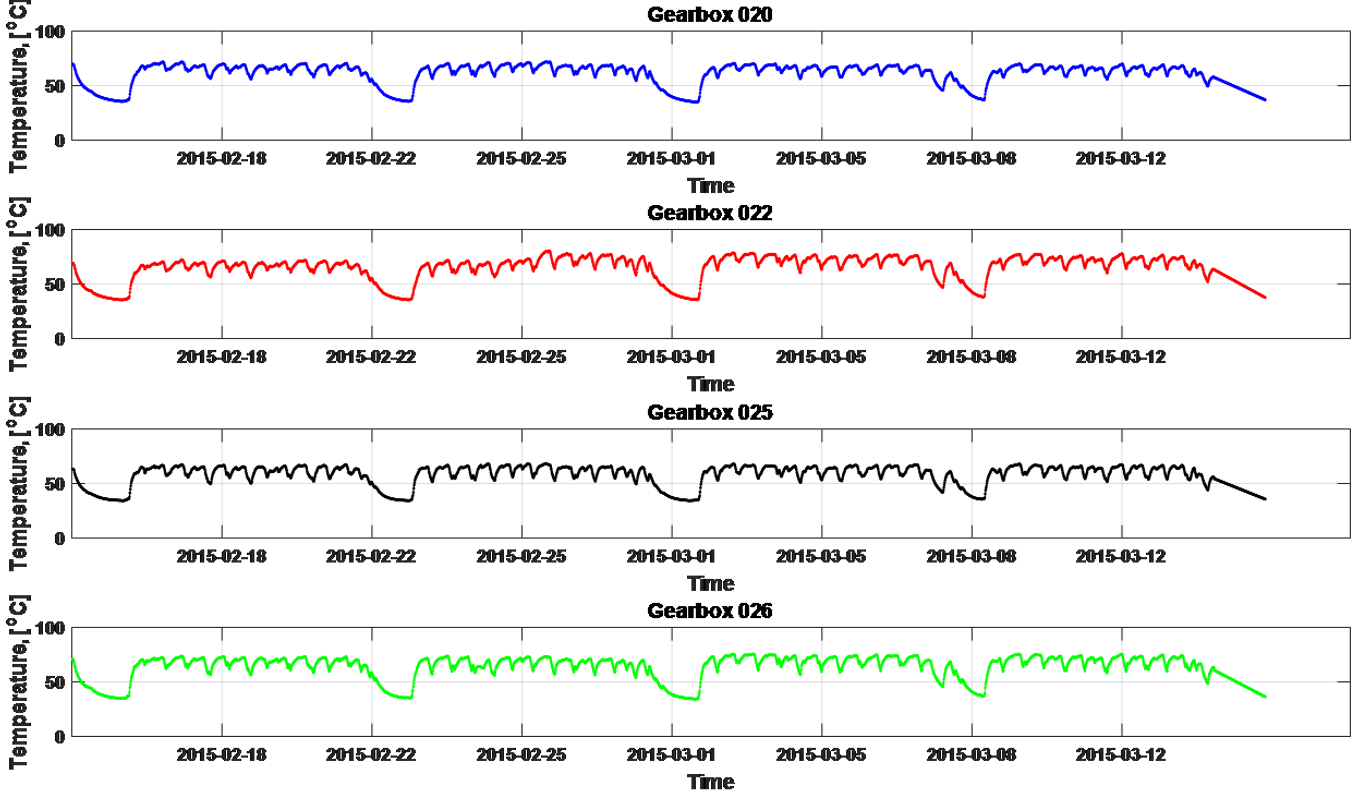
\includegraphics[width = 0.8\textwidth]{wykresy/ica_raw.png}
\caption{Preprocessed input signals.}
\label{fig: ica_raw}
\end{figure}

At first, signals had to~be preprocessed according to~methodology described in~section \ref{temp_ica}, and the~output sampling period was set to~15 minutes. First conclusion when comparing Fig \ref{fig: ica_raw} is~that looking of~each signal separately is~non-effective from diagnostic point of~view. 

% \begin{figure}[ht!]
% \centering
% 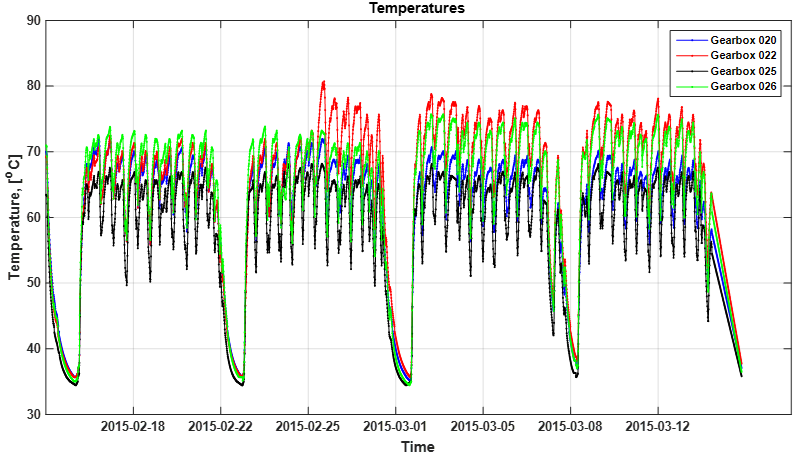
\includegraphics[width = 1\textwidth]{wykresy/ica_raw2.png}
% \caption{Signals presented together.}
% \label{fig: ica_raw2}
% \end{figure}

However, an~automatic technique is~required, that will allow to~extract process related to~change of~condition only. Hence, ICA approach was used. In this case ICA returns four features with estimated unmixing matrix $W^T$:

\begin{gather}
 W^T =
 \begin{bmatrix}
  0,469 & 0,006 & -0,504 & 0,076 \\
  -0,104 & -0,151 & -0,586 & 0,725 \\
  -0,304 & 0,335 & -0,035 & -0,019 \\
  -0,343 & -0,163 & 0,417 & 0,165
  \end{bmatrix}
\end{gather}

For reasons described in~section \ref{app_ica} arrangement of~output features will be~different every time. As we can see in~Fig. \ref{fig: ica_feat} features 1 and 4 carry information about common factors of~signals behavior, feature 2 presents highest frequency details, and feature 3 informs about trend of~behavior change, so in~this case third feature is~selected for further analysis. Besides, cross-correlation provides the~information that selected feature is~connected with behavior of~signal coming from gearbox 022.

\begin{figure}[ht!]
\centering
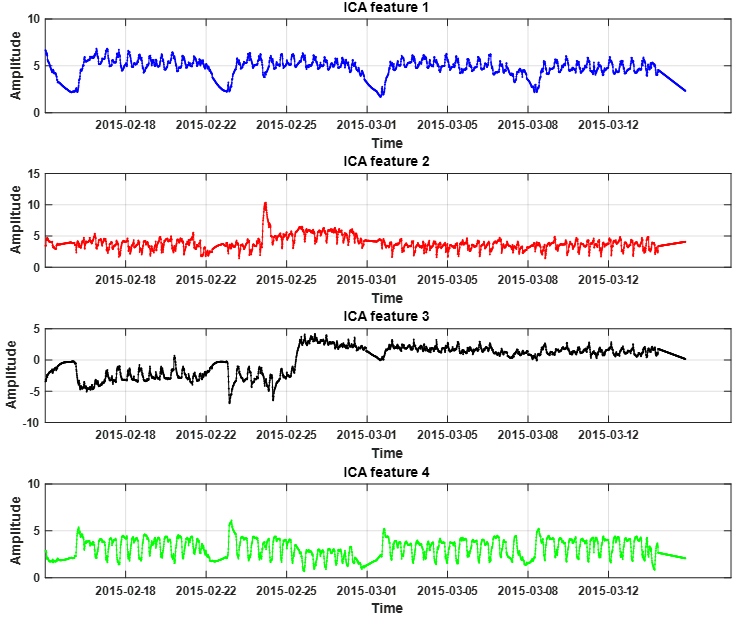
\includegraphics[width = 0.7\textwidth]{wykresy/ica_feat.png}
\caption{Four features obtained from ICA.}
\label{fig: ica_feat}
\end{figure}

Selected feature along with daily variances is~presented in~Fig. \ref{fig: ica_feat2}. One can see that two events can cause an~alarm. Event occurring during $12^{th}$ day can be~clearly visible in~the~third feature in~Fig. \ref{fig: ica_feat}. The event originates from the~signal from gearbox 022. On the~other hand, event occurring during $9^{th}$ day is~not easily visible. Fig. \ref{fig: ica_feat3} presents this situation. One can see that during $24^{th}$ of~February, temperature of~gearboxes 026 and 022 dropped unusually compared to~behavior from previous work cycles. 

\begin{figure}[ht!]
\centering
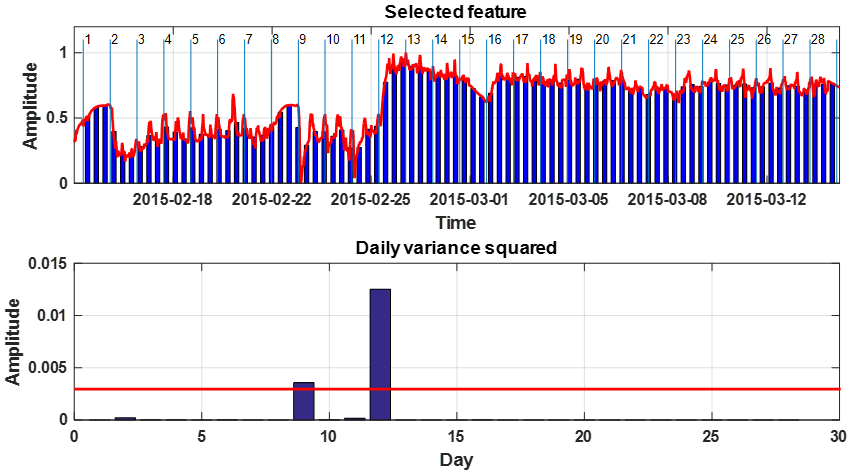
\includegraphics[width = 0.7\textwidth]{wykresy/ica_feat2.png}
\caption{Selected feature with consecutive days indicated. Daily variance squared has been proposed as~event selector.}
\label{fig: ica_feat2}
\end{figure}

\begin{figure}[ht!]
\centering
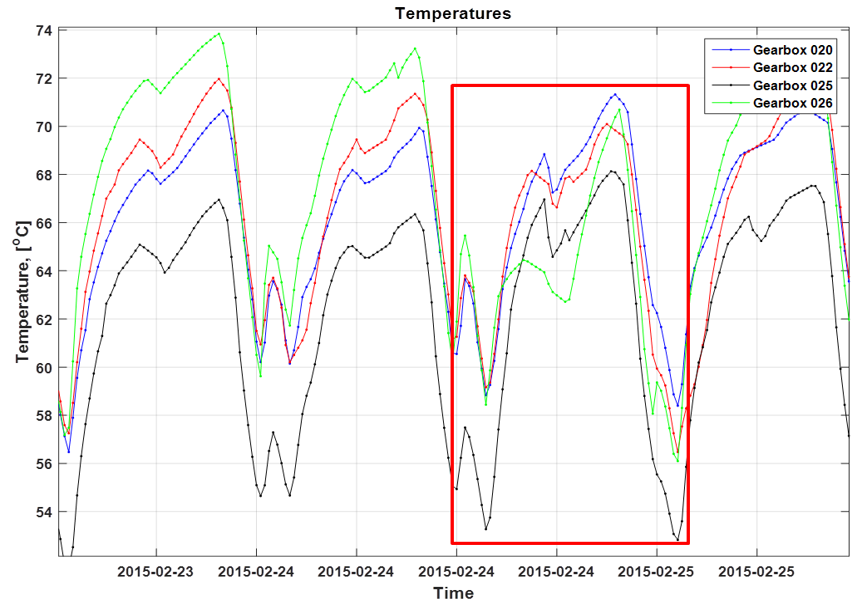
\includegraphics[width = 0.6\textwidth]{wykresy/ica_feat3.png}
\caption{Event from day 9. The unusual temperature drop on~the~gearboxes 026 and 022 also triggered the~warning indicator.}
\label{fig: ica_feat3}
\end{figure}

% \subsubsection{Summary}

% In this paper author presented application of~Independent Component Analysis for signal feature extraction applied to~real temperature signal from set of~heavy duty gearboxes used in~mining industry. The methodology is~based on~the~analysis of~multichannel time series. In order to~extract information about the~damage author analyzed the~features obtained by~applying the~ICA to~four-channel input signal. Extracted features allow to~detect unusual behavior of~gearboxes, identify misbehaving device and provide behavioral feature for further analysis and interpretation. By using ICA author was able to~separate different sources influencing shape of~measured temperature signal, or in~other words, it~is~possible to~remove contribution related to~operational factors from the~signal.

\subsection{Work regimes distinction using EM}\label{result_em}

In this section author describes how method presented in~section \ref{temp_em} was used to~analyze temperature data measured on~a~single heavy-duty gearbox used in~belt conveyor driving station in~underground mine.

Parameterization using selected statistics allowed to~construct three feature vectors presented in~the~Fig. \ref{fig: cluster_stats_day}

\begin{figure}[ht!]
\centering
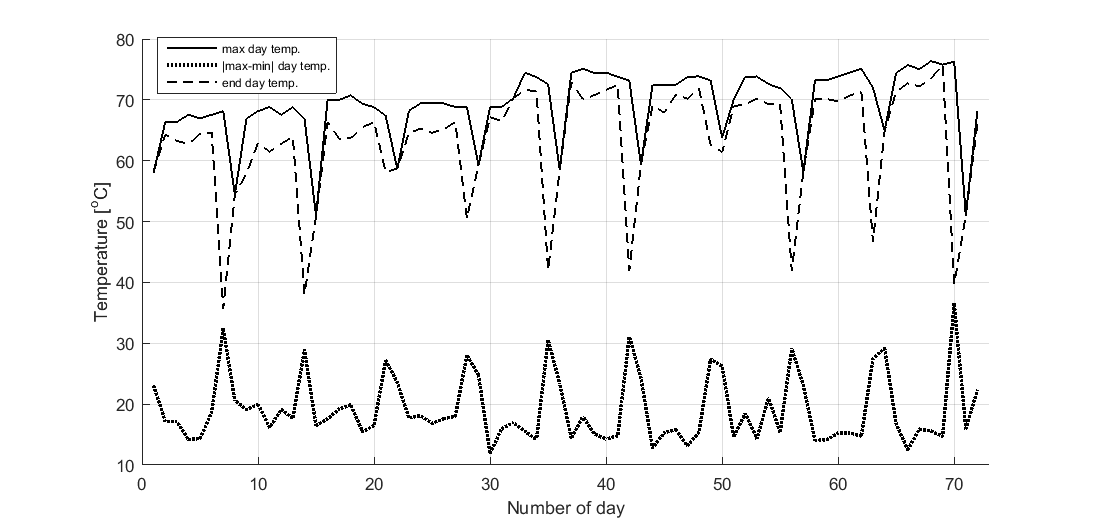
\includegraphics[width = \textwidth]{wykresy/cluster_stats_day.png}
\caption{Vectors of~statistics used in~clustering process.}
\label{fig: cluster_stats_day}
\end{figure}

Three-dimensional data points constructed from described statistic vectors distributed themselves in~the~3D feature space as~shown in~Fig \ref{fig: unclusteredbw}. It is~clearly visible that there are four or even five clusters possible to~be distinguished. For this dataset Silhouette criterion returned optimal amount of~clusters equal to~$5$ (see definition in~section \ref{app_sil}). As a~result of~presented procedure author obtained information about individual days belonging to~certain clusters (see Fig. \ref{fig: clustered}). Each cluster defines in~correct and accurate way one of~five possible outcomes:

\begin{figure}[ht!]
\centering
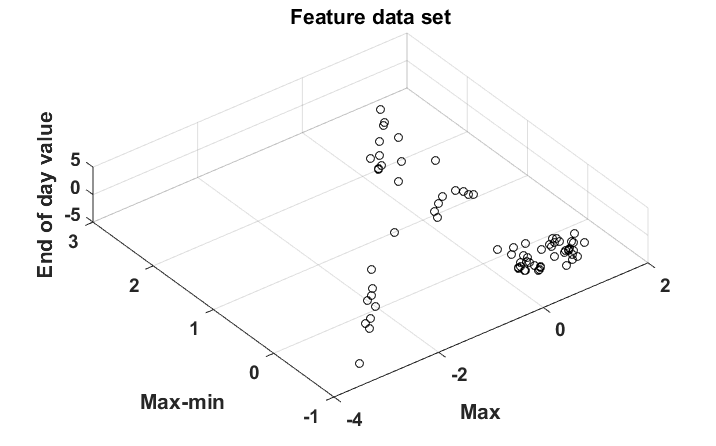
\includegraphics[width = \textwidth]{wykresy/unclusteredbw.png}
\caption{Distribution of~points in~3D feature space.}
\label{fig: unclusteredbw}
\end{figure}

\begin{itemize}
\renewcommand{\labelitemi}{$\bullet$}
\item Mondays,
\item Saturdays,
\item Sundays,
\item Other days of~the~week in~good condition,
\item Other days of~the~week in~bad condition.
\end{itemize}

All of~those classes are important to~be detected and identified. Mondays, Saturdays and Sundays reveal very outlying behavior, hence they are not informative and are detected only to~be eliminated from further analysis. On the~other hand, theoretically all days of~the~week could be~divided into classes of~good and bad conditions, but it~was impossible for such limited amount of~data. Longer data record might cause points in~feature space to~fill cavities within the~clusters. Because of~that, point clouds would be~denser and more consistent. It would allow the~Silhouette criterion to~estimate larger optimal cluster amount, which then could possibly lead to~distinction between good and bad condition on~Mondays, Saturdays and Sundays.

\begin{figure}[ht!]
\centering
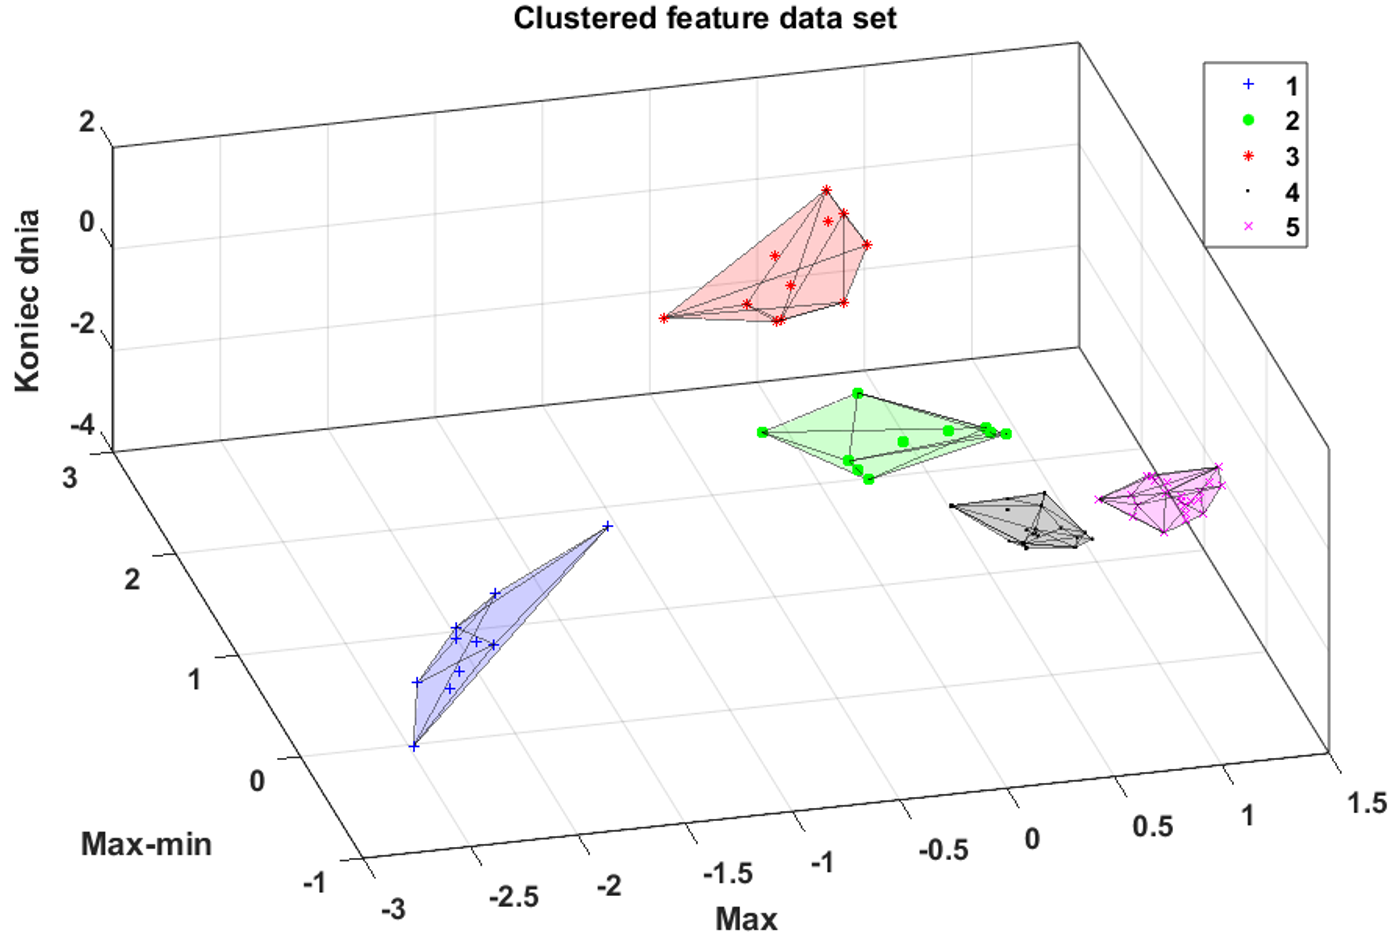
\includegraphics[width = \textwidth]{wykresy/clustered.png}
\caption{Clustering results in~feature space (values normalized). Clusters represent Sundays (1), Saturdays (2), Mondays (3), other days in~good condition (4), and other days in~bad condition (5).}
\label{fig: clustered}
\end{figure}

Fig. \ref{fig: cplot} presents the~results in~time domain. One can clearly see that EM algorithm correctly assigned particular days to~their respective classes.

\begin{figure}[ht!]
\centering
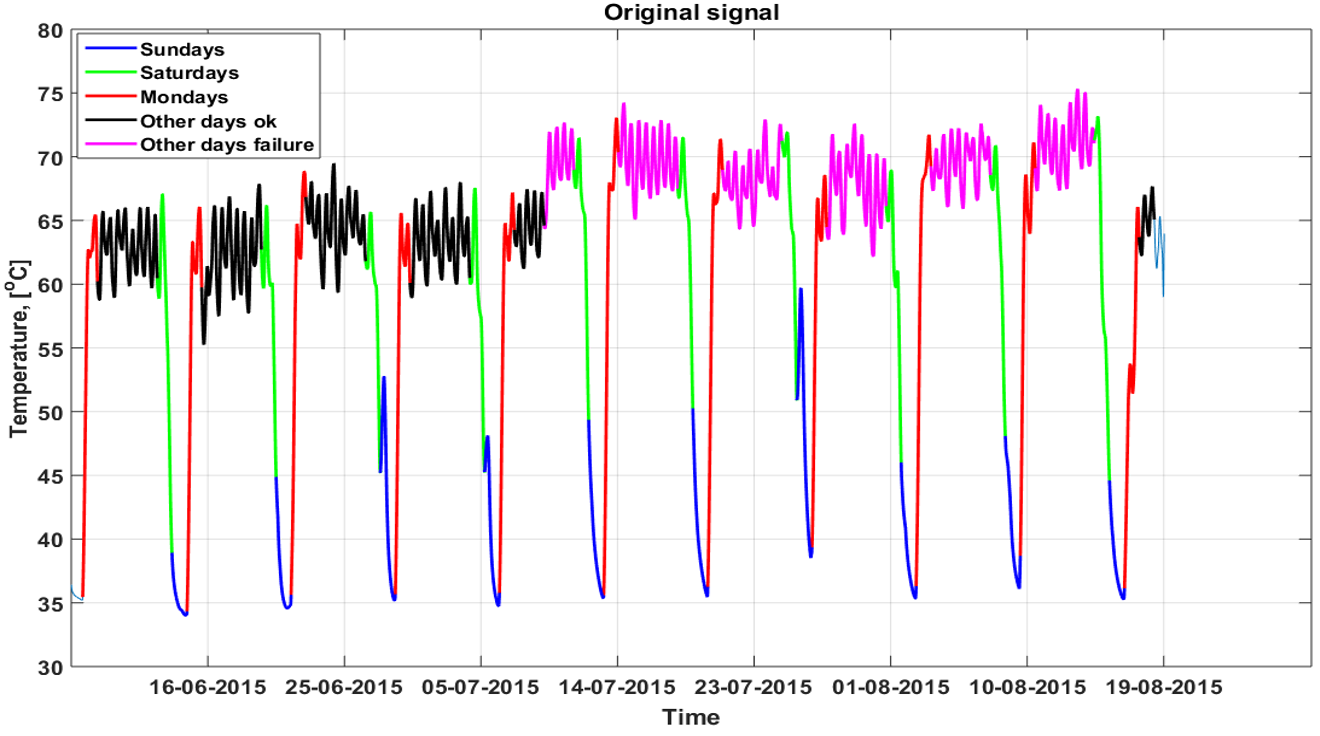
\includegraphics[width = \textwidth]{wykresy/cplot.png}
\caption{Clustering results in~time domain.}
\label{fig: cplot}
\end{figure}

\subsection{Time-time map analysis for LHD fault detection}\label{real_bulgaria}

\subsubsection{Data description}

Measured data originate from the~built-in data acquisition system provided by~the~manufacturer of~LHD machines. In this work author focused only on~one variable describing temperature of~engine coolant. Data has been provided with sampling period of~30 seconds, which is~enough in~case of~slowly varying values such as~temperature. Data describes period of~about two and a~half months (see Fig. \ref{fig: lhd_temp_raw}).

\begin{figure}[ht!]
\centering
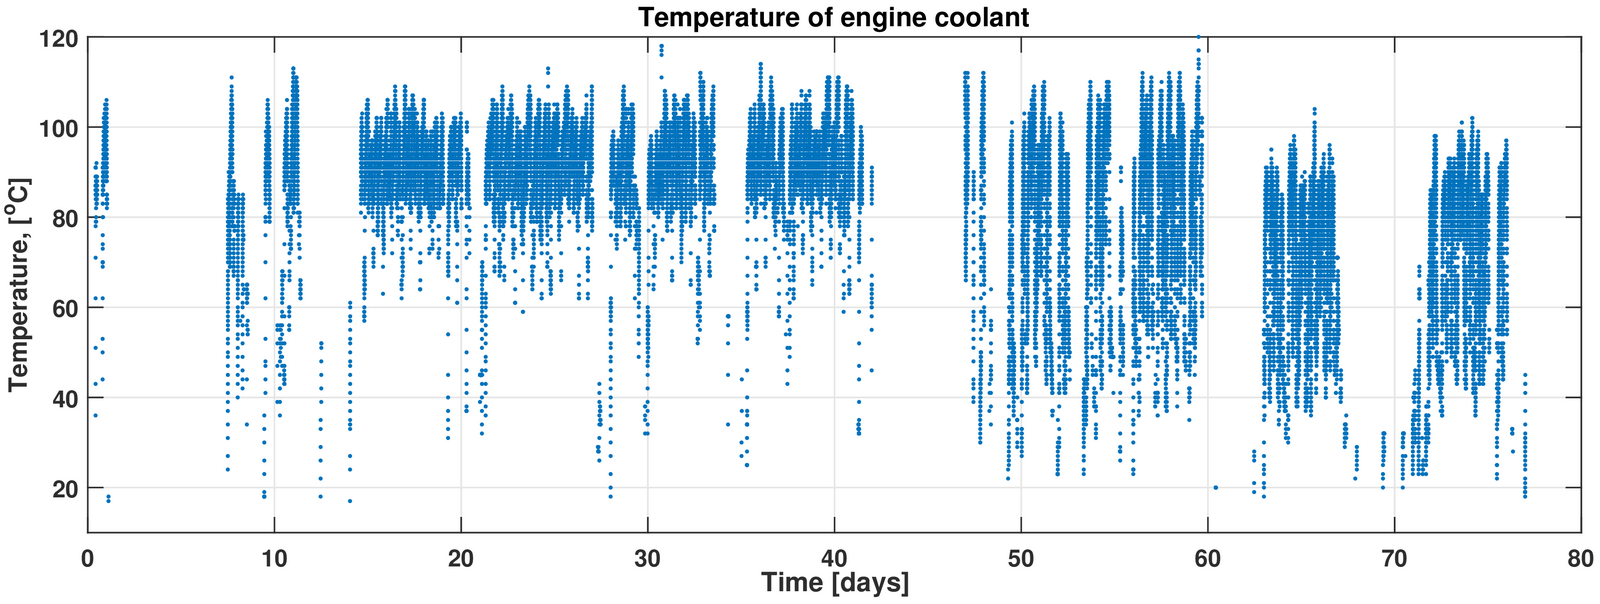
\includegraphics[width = \textwidth]{wykresy/lhd_temp_raw.png}
\caption{Raw time series of~input data.}
\label{fig: lhd_temp_raw}
\end{figure}

According to~preprocessing described in~section \ref{temp_bulgaria} data has been transformed to~time-time representation (see Fig. \ref{fig: lhd_temp_map}).

\begin{figure}[ht!]
\centering
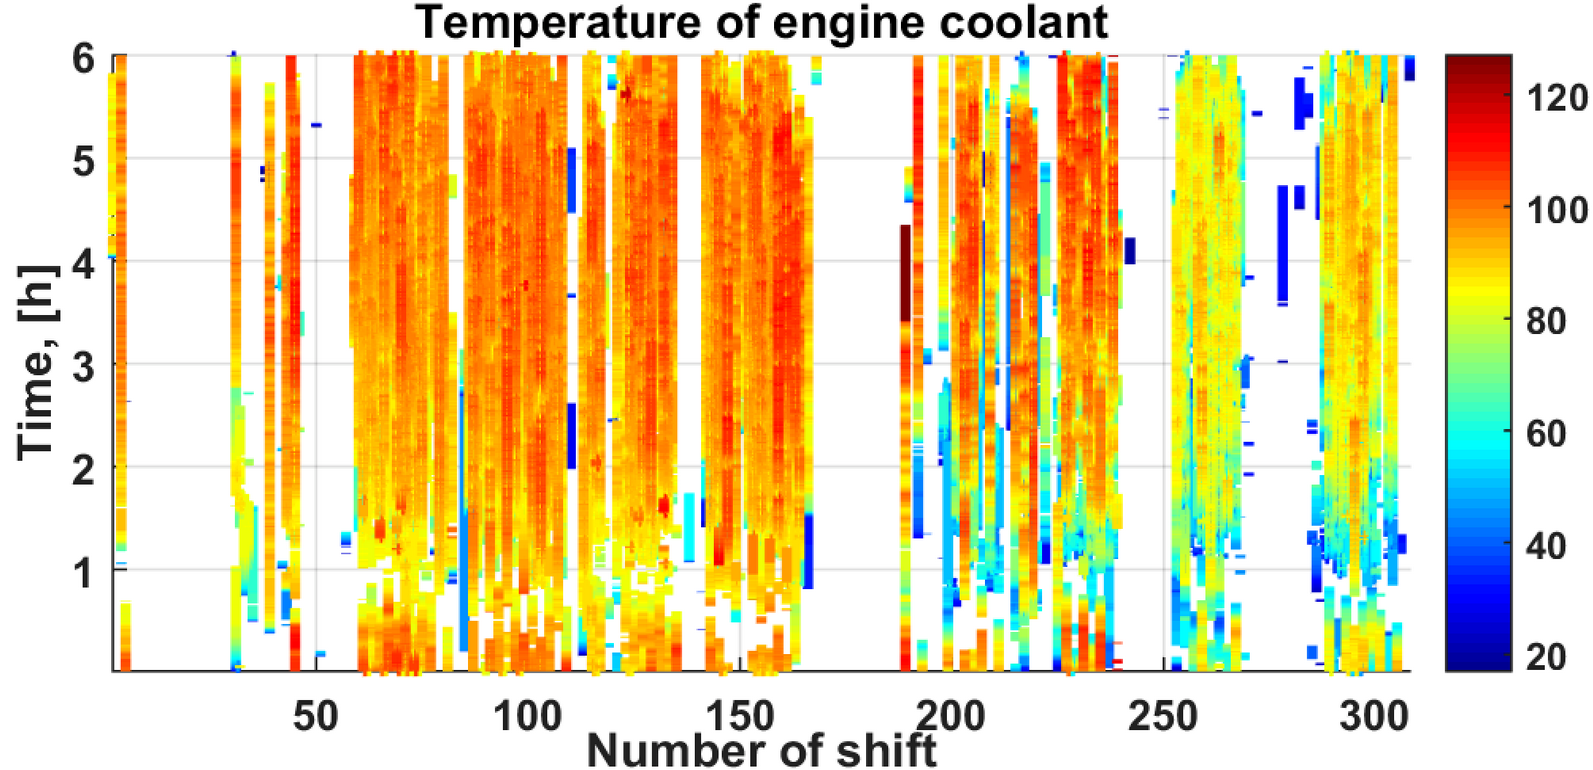
\includegraphics[width = \textwidth]{wykresy/lhd_temp_map.png}
\caption{Map of~engine coolant temperature values along consecutive shifts. Colors represent temperature values.}
\label{fig: lhd_temp_map}
\end{figure}

After disregarding empty and nearly empty work shifts (see Fig. \ref{fig: lhd_temp_map2}) the~first step was to~calculate probability density map and smooth it. Fig. \ref{fig:ks_maps} presents probability density maps: raw (left panel) and smoothed (right panel).

\begin{figure}[ht!]
\centering
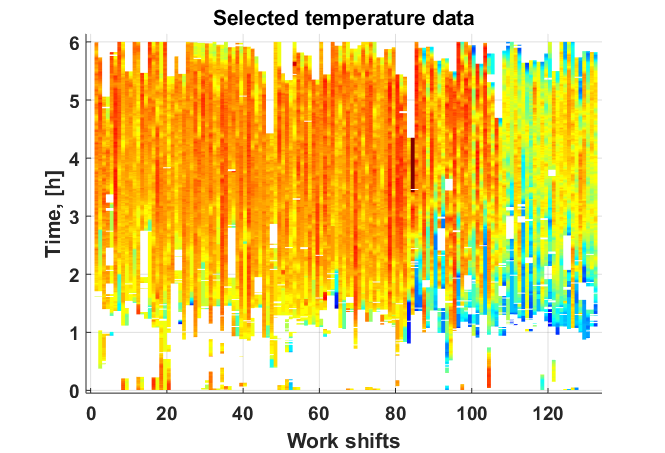
\includegraphics[width = 0.8\textwidth]{wykresy/lhd_temp_map2.png}
\caption{Remaining temperature data after selection.}
\label{fig: lhd_temp_map2}
\end{figure}

\begin{figure}[!ht]
 \centering
 \begin{subfigure}
   \centering
   % \captionsetup{skip=0.01pt}
   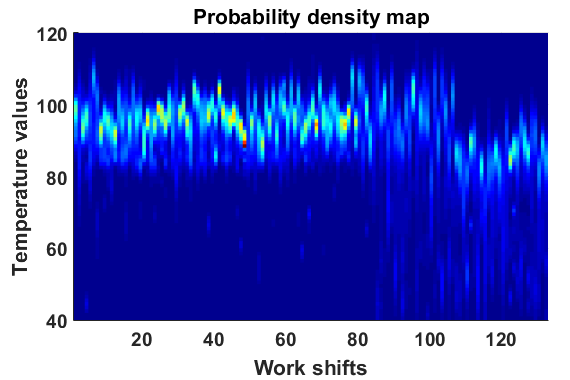
\includegraphics[width=0.49\textwidth]{wykresy/ks_map.png}
  %  \caption{Input data in~time-time domain}
   \label{fig:ks_map}
 \end{subfigure}
 %\hfill
 \begin{subfigure}
   \centering
  % \captionsetup{skip=0.01pt}
		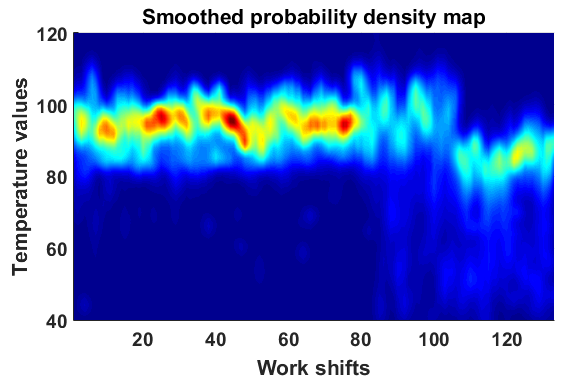
\includegraphics[width=0.49\textwidth]{wykresy/ks_map2.png}
    % \caption{Selected interpolated shifts}
  \label{fig:ks_map2}
 \end{subfigure}
 \caption{Probability density map created from raw data (left panel) and smoothed map (right panel). Smoothing the~data results in~more consistent behavior of~the~calculated statistics.}
 \label{fig:ks_maps}
\end{figure}

It can be~easily seen that data is~divided into three main health states that change at~two points: at~about $80^{th}$ shift and at~about $110^{th}$ shift counting according to~the~density map. First state is~characterized with relatively low dispersion of~data values as~well as~overall symmetry and stability of~data distributions. 

\begin{figure}[ht!]
\centering
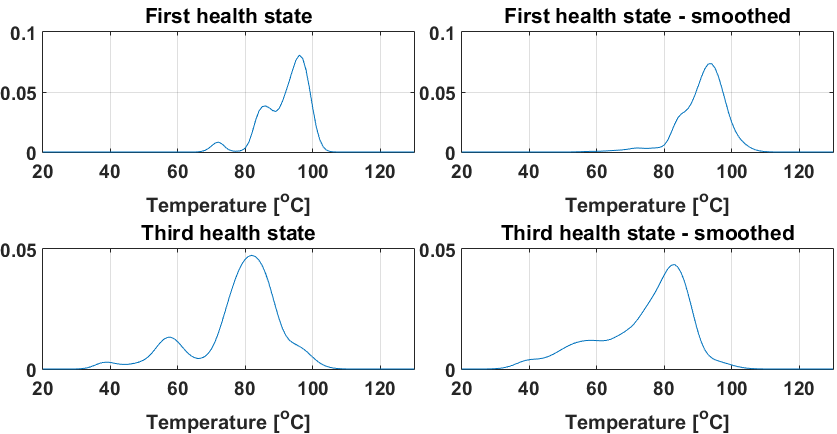
\includegraphics[width = 0.8\textwidth]{wykresy/ks_ex.png}
\caption{Examples of~density functions selected from first health state (top panels) and third health state (bottom panels) drawn from raw density map (left panels) and smoothed density map (right panels).}
\label{fig: ks_ex}
\end{figure}

The second one reveals sudden increase of~data dispersion with appearance of~negative skewness of~the~distributions with preservation of~fundamental mode position. Third state also indicates negative skewness and higher dispersion than the~first one, but fundamental mode of~the~distributions is~shifted significantly towards lower values. It is~clearly visible that difference between density functions from different health states is~significant and can allow to~identify and segment health states (see Fig. \ref{fig: ks_ex}).

\begin{figure}[ht!]
\centering
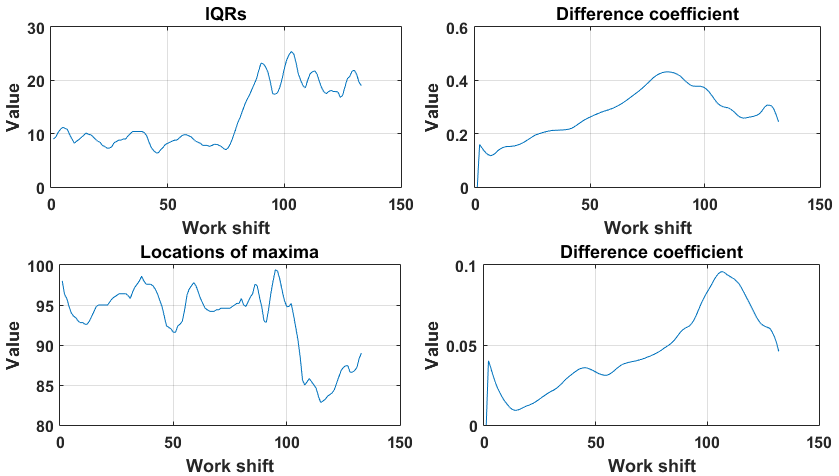
\includegraphics[width = 0.8\textwidth]{wykresy/ks_stats.png}
\caption{Operational statistics (left panels) and their difference coefficients (right panels).}
\label{fig: ks_stats}
\end{figure}

Calculated statistics and their difference coefficients are shown on~Fig. \ref{fig: ks_stats}. In practice author calculated this coefficient for every splitting point, and then found the~maximum of~such vector. It can be~seen that each statistic clearly indicates one of~regime shifts in~the~data.

\begin{figure}[ht!]
\centering
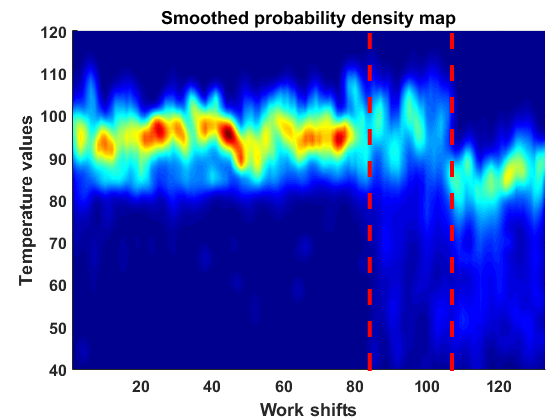
\includegraphics[width = 0.6\textwidth]{wykresy/ks_map3.png}
\caption{Localized regime shifts presented on~density map.}
\label{fig: ks_map3}
\end{figure}

Regime shifts have been localized and overlaid on~probability density map (see Fig. \ref{fig: ks_map3}) and on~original temperature time series (see Fig. \ref{fig: ks_final}). For this data sample they were identified to~be shifts no. $189$ and $253$ counting within all shifts before empty values removal, or shifts no. $84$ and $107$ counting according to~density map. 

It is~very important to~mention that accounting system of~the~mine reports the~repair performed on~the~machine on~the~day $108$, that was connected to~the~engine overheating problem. 

\begin{figure}[ht!]
\centering
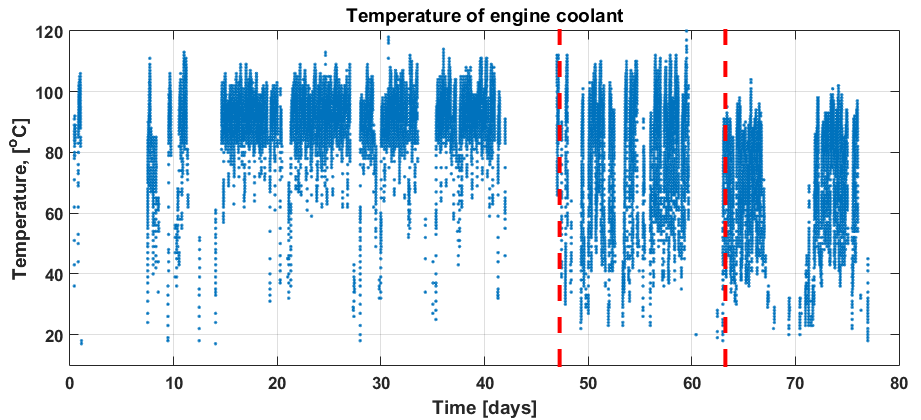
\includegraphics[width = \textwidth]{wykresy/ks_final.png}
\caption{Localized regime shifts presented on~raw data.}
\label{fig: ks_final}
\end{figure}

Considering that presented method uses data smoothing and probabilistic techniques that can in~theory decrease precision of~calculations, difference of~only one day between date of~second found regime shift and date of~reported repair is~surprisingly small, and concludes high quality of~the~method. Presented method correctly identifies changes in~characteristics of~operation, basing on~the~temperature data of~engine coolant. Tracking and interpretation of~those changes might be~used to~prepare preventive maintenance scenarios for the~machine, and prolong its lifespan in~the~long run. 

\subsection{Anderson-Darling statistic map for failure detection}\label{real_ad}

In this section presented method described in~section \ref{temp_ad} is~applied to~real-life temperature data. Method is~operating on~data already described in~section \ref{real_bulgaria}, and preprocessing stage that constructs time-time representation is~identical (see Fig. \ref{fig: lhd_temp_map2}).

\begin{figure}[!ht]
 \centering
 \begin{subfigure}
   \centering
   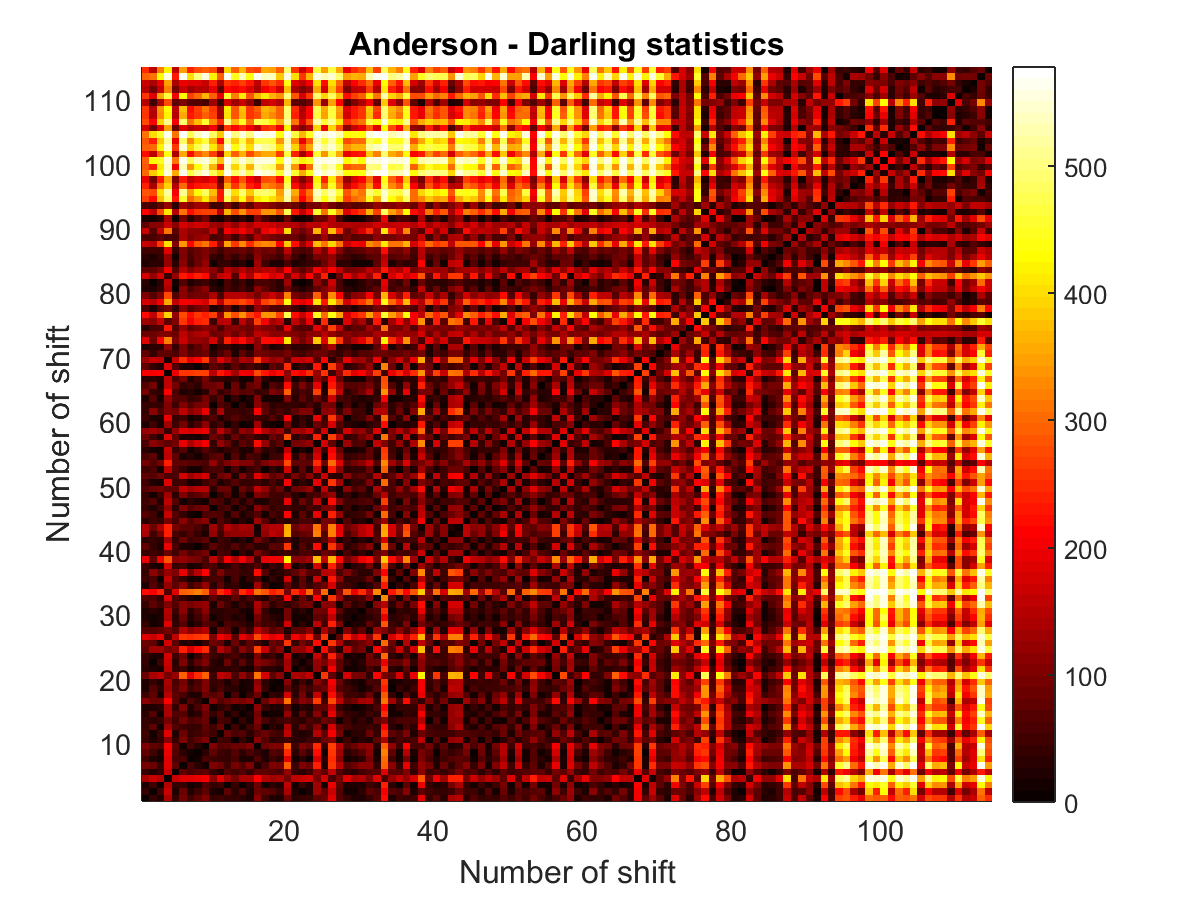
\includegraphics[width=0.48\textwidth]{wykresy/ADK-stat}
 \end{subfigure}
 \begin{subfigure}
   \centering
		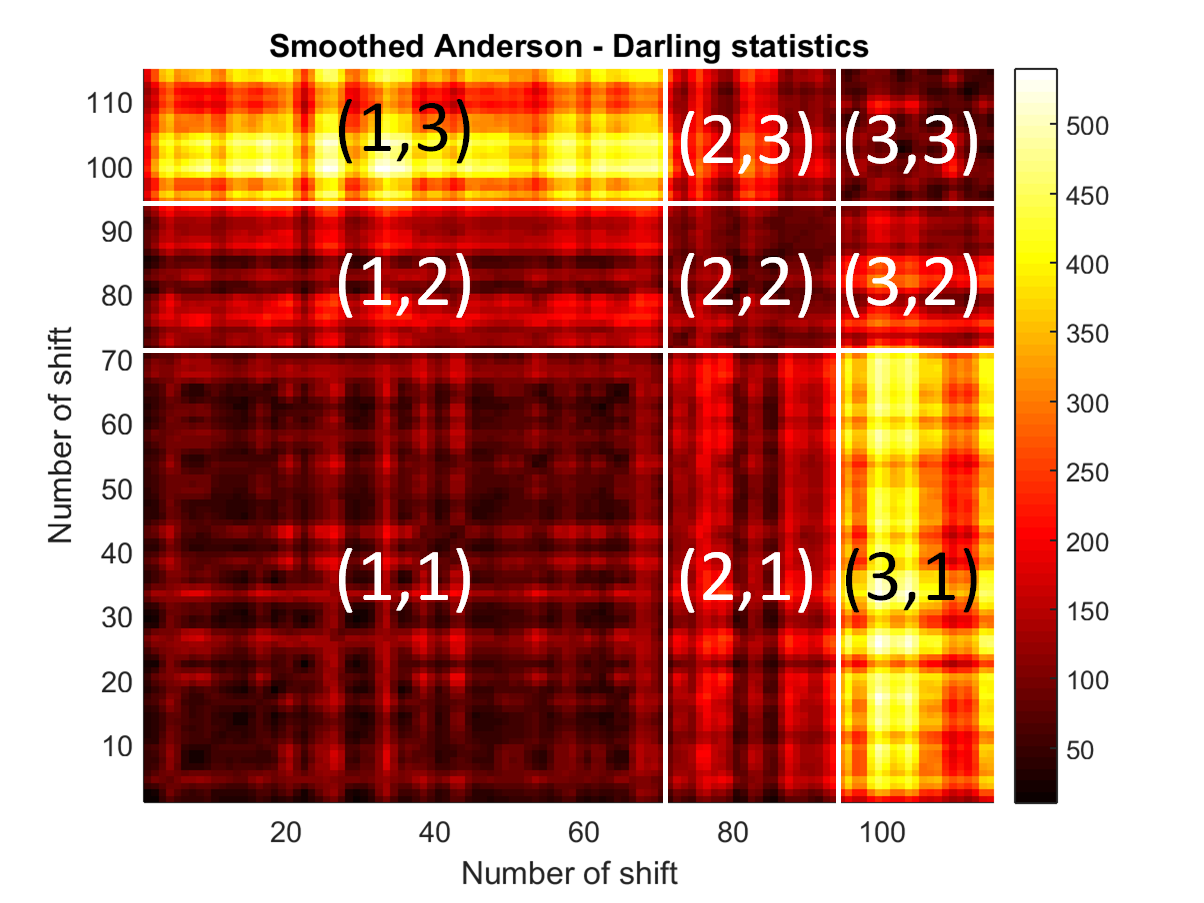
\includegraphics[width=0.48\textwidth]{wykresy/ADK-stat-smooth2}
 \end{subfigure}
 \caption{Anderson-Darling statistic map (left panel) and the~same map after filtering with triangular kernel (right panel) with notation corresponding to~Fig. \ref{fig:map}}
 \label{fig:ADK-stat-2}
\end{figure}

Left panel of~Figure \ref{fig:ADK-stat-2} shows the~values of~Anderson-Darling statistics for each pair of~compared work shifts. Areas connected to~described processes are visible, but after filtration properties of~the~map are enhanced (see Fig. \ref{fig:ADK-stat-2} right panel).

\begin{figure}[!ht]
 \centering
 \begin{subfigure}
   \centering
   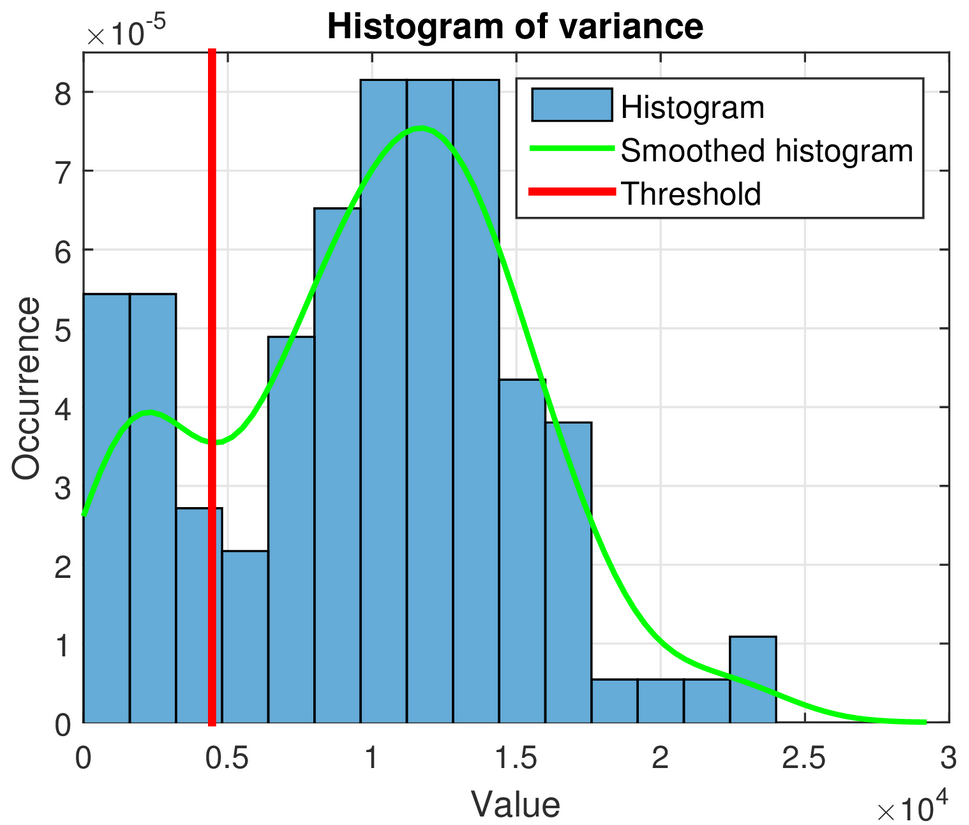
\includegraphics[width=0.48\textwidth]{wykresy/ksd}
 \end{subfigure}
 \begin{subfigure}
   \centering
		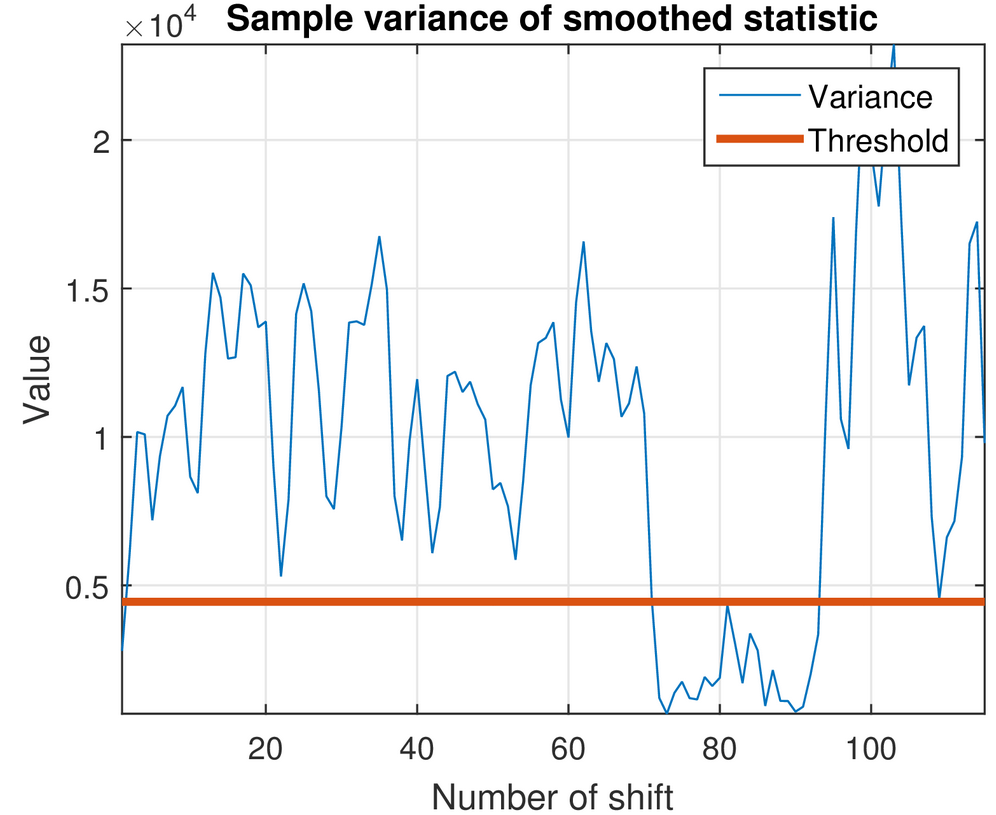
\includegraphics[width=0.48\textwidth]{wykresy/ADK-thr}
 \end{subfigure}
 \caption{One-dimensional sample variance of~filtered AD map thresholded by~local minimum of~smoothed histogram of~the~variance vector}
 \label{fig:ADK-KS-thr}
\end{figure}

After filtering AD map, sample variance of~column vectors is~calculated. The values of~variance for each work shifts are presented in~right panel of~Fig. \ref{fig:ADK-KS-thr} (blue line). Next step is~to~estimate its distribution by~smoothed histogram and calculate local minimum of~this function (see left panel of~Fig. \ref{fig:ADK-KS-thr}). Author proposes to~take this value as~a~threshold (red line in~right panel of~Fig. \ref{fig:ADK-KS-thr}). The area where variance is~smaller that threshold corresponds with failure state.

Transition points have been overlaid on~input temperature data (see Fig. \ref{fig: AD_final}). They were identified to~be at~shifts no. 166 and 238 when counting within all shifts before empty values removal, or shifts no. 72 and 93 when according to~interpolated map. It is~important to~mention that accounting system of~the~mine reports the~repair performed on~the~machine, that was connected to~the~engine overheating problem. The actual day of~repair is~the~day after detected change of~technical condition. Considering that method presented in~this paper based on~statistical analysis, smoothing and transforming from two to~one-dimensional form has only one day difference between date of~reported repair and date of~second found transition point is~surprisingly small.

\begin{figure}[ht!]
\centering
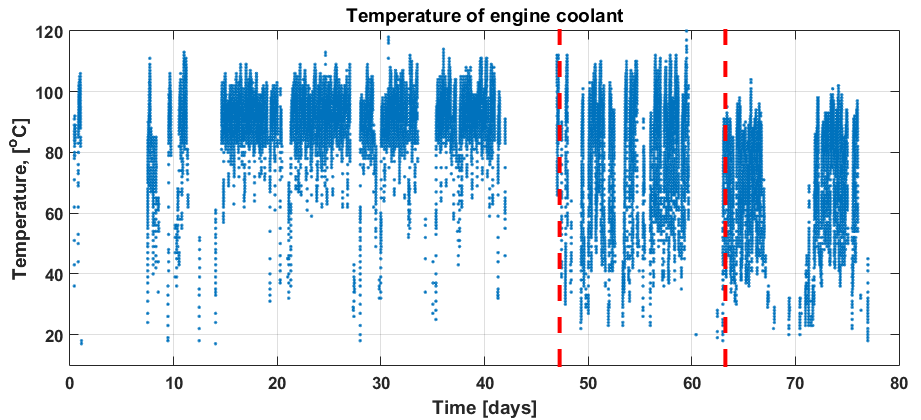
\includegraphics[width = \textwidth]{wykresy/ks_final.png}
\caption{Localized regime shifts presented on~raw data.}
\label{fig: AD_final}
\end{figure}

As a~result, long-term observation has been divided into three health states: warning state (approaching failure), state of~failure and healthy state after repair. Localized moments of~state changes have been positively verified with experts from the~mine, which confirms correctness of~obtained results and overall method performance.


\clearpage
\section{Muiltichannel spectrogram analysis using PCA}\label{result_pca}

In this section presented method described in~section \ref{met_pca} is~applied to~real-life multichannel vibration data.

\subsubsection{Data description}

The machine considered here is~a~two-stage gearbox used in~drive system for belt conveyor. Raw multichannel signal and its spectrogram representation is~shown in~Fig. \ref{fig: pca_raw} and \ref{fig: pca_spec}, respectively. Both time series and their spectrograms allow to~notice some weak impulsive/wideband components but it~is~impossible to~be distinguished unambiguously.


% The experiment shows that the~gearbox does not reveal any damage. Thus, an~artificial damage is~introduced by~specific signal processing technique in~order to~illustrate benefits of~the~proposed methodology. Namely, each of~four acquired signals is~considered as~a~response of~the~system (each signal stands for an~individual system) to~stationary noise, since there is~no damage in~the~gearbox. Thus, we fit the~autoregressive (AR) model to~each of~four signals by~Yule-Walker equations and obtain four sets of~coefficients called the~impulse responses of~the~system. Orders of~the~AR models are high enough to~reflect complexity of~amplitude spectra of~the~acquired signals. Then, four pulse trains (Kronecker combs) with additive Gaussian noise are designed as~excitation signals (source signals) that correspond to~a~damaged gearbox. Duration of~the~excitation signals is~equal to~the~duration of~signals acquired during the~experiment. The fault frequency associated to~damage in~gear-wheel on~the~middle shaft is~4.1 Hz and this is~the~frequency of~impulses in~the~pulse trains. The ratio of~impulse to~noise amplitudes is~different for each excitation signal, which corresponds to~different distance between each sensor and the~damaged gear. Finally, the~pulse trains are convolved with corresponding impulse responses and such signals are further analyzed and referred as~“raw signals”.

\begin{figure}[ht!]
\centering
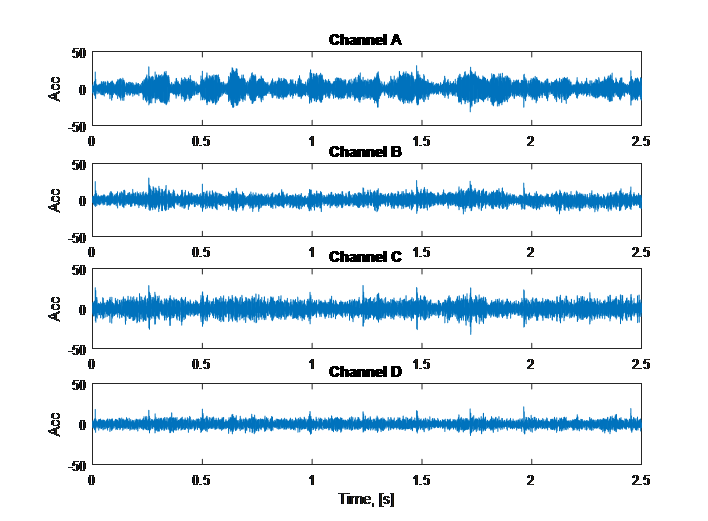
\includegraphics[width = 0.8\textwidth]{wykresy/pca_raw.png}
\caption{Multichannel input signal.}
\label{fig: pca_raw}
\vspace{-10px}
\end{figure}


\begin{figure}[ht!]
\centering
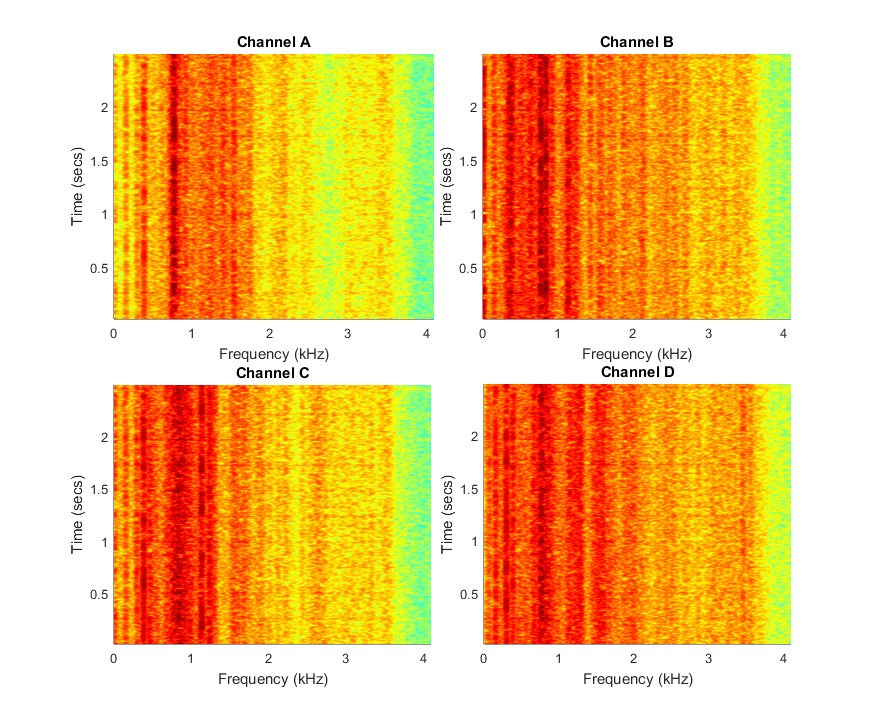
\includegraphics[width = 0.8\textwidth]{wykresy/pca_spec.png}
\caption{Spectrograms of~input signal.}
\label{fig: pca_spec}
\end{figure}

\subsubsection{Results}

In this section author presents the~results of~introduced method, i.e. performance of~the~algorithm fed with discussed data. Fig. \ref{fig: pca_out} (left panel) presents new time-frequency map which consists of~the~components extracted by~applying PCA to~the~sub-signals from the~initial spectrograms. The impulses (wideband excitations) are visible much more clearly than in~the~spectrograms of~multichannel raw signal (see Fig. \ref{fig: pca_spec}). Moreover, simple aggregation of~2D map into 1D vector by~integration of~energy for each time instance shows impulsive nature of~energy flow. Using simple spectrum one can identify period/frequency of~impulse repetition that corresponds to~fault frequency, see Fig. \ref{fig: pca_out} (right panel).

It is~also important to~note that scores of~principal components of~slices from initial spectrograms vary in~frequency domain. Although always first component was taken, its score ranged from over 0.99 for heavily impulsive frequency bins, down to~less than 0.6 for bins that did not carry as~much impulsive information.

\begin{figure}[!ht]
 \centering
 \begin{subfigure}
   \centering
   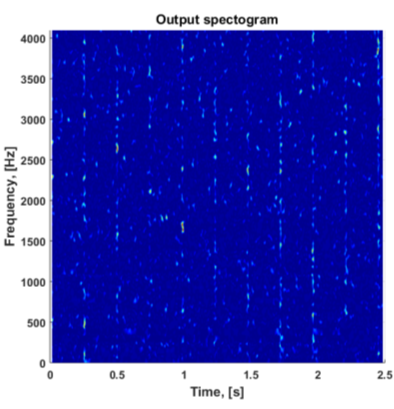
\includegraphics[width=0.48\textwidth]{wykresy/pca_outspec.png}
 \end{subfigure}
 \begin{subfigure}
   \centering
		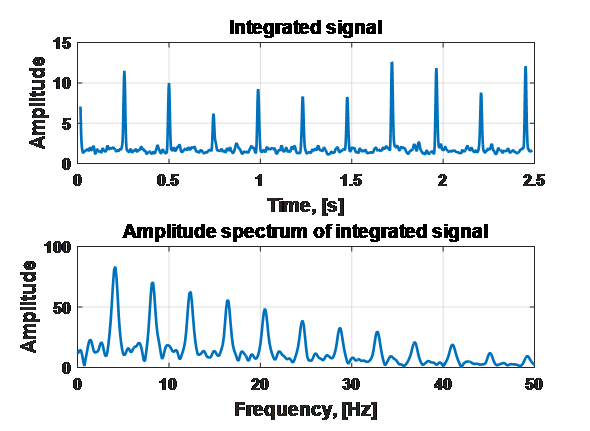
\includegraphics[width=0.48\textwidth,height=0.48\textwidth]{wykresy/pca_outts.png}
 \end{subfigure}
 \caption{Output spectrogram composed of~first PCA components (left panel). Right panels: Time series extracted from output spectrogram and spectrum of~integrated time series.}
 \label{fig: pca_out}
\end{figure}


\clearpage
\section{Methods for multidimensional domain analysis using NMF algorithms}

\subsection{STFT analysis taking advantage of~NMF encoding matrix}\label{result_enc}

In this section, author focuses on~the~analysis of~vibration data captured on~rolling bearing of~the~drive pulley according to~the~methodology described in~section \ref{met_nmf_enc}. In Fig. \ref{fig: nmf_raw} time series of~signal recorded on~the~faulty pulley bearing is~presented, and Fig. \ref{fig: nmf_spec} shows the~spectrogram of~the~signal. This data has been already analyzed in~recent papers, where several methods for local damage diagnostics have been proposed, see review in~[18]. The sampling frequency is~equal to~19.2 kHz and the~measurement is~2.5 seconds long. The spectrogram is~obtained for the~Hamming 512-sample length window with 450 overlapping samples and 512 FFT points. 

% One can notice several wide-band excitations on~the~spectrogram at~carrier frequency band 1-6 kHz that occur with the~modulation frequency of~12.7 Hz (and its multiples). This stands for outer race local damage.

\begin{figure}[ht!]
\centering
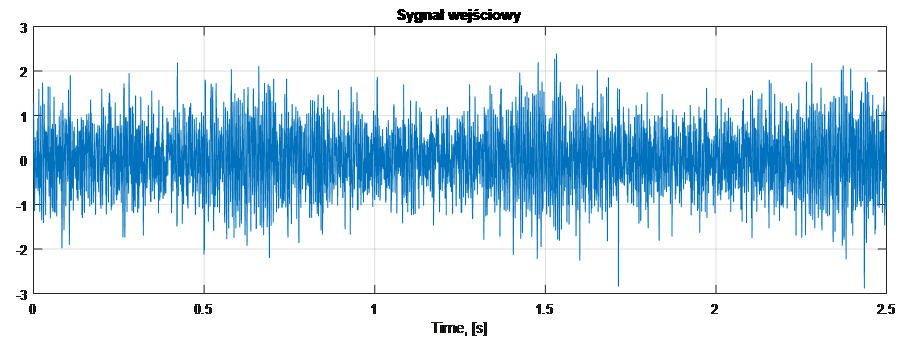
\includegraphics[width = 0.8\textwidth]{wykresy/nmf_raw.png}
\caption{Raw input signal.}
\label{fig: nmf_raw}
\end{figure}

\begin{figure}[ht!]
\centering
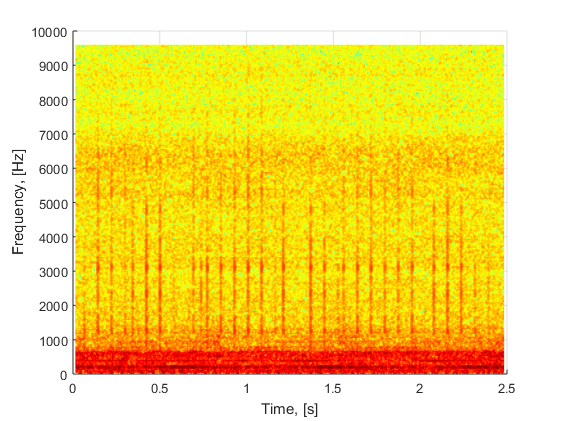
\includegraphics[width = 0.7\textwidth]{wykresy/nmf_spec.png}
\caption{Spectrogram of~input signal.}
\label{fig: nmf_spec}
\end{figure}

As a~next step, Semi-binary NMF algorithm groups the~spectra into three clusters (see Fig. \ref{fig: nmf_partial}) which are then transformed back to~time-series form using bulit-in Matlab procedure \texttt{istft} for Short-Time Fourier Transform inversion. Third cluster is~selected for further analysis based visual inspection (manually) or based on~maximum kurtosis of~obtained signals (automatically). The selected signal has zero value everywhere except for places where impulses occur (see Fig. \ref{fig: nmf_out} a). In those places ISTFT produced portion of~the~signal that comes from the~spectrogram slices assigned to~a~particular place (typically 3-8 slices per impulse), and hence they carry information from the~original signal (slightly suppressed by~ISTFT windowing, see Fig. \ref{fig: nmf_imp} a).

\begin{figure}[ht!]
\centering
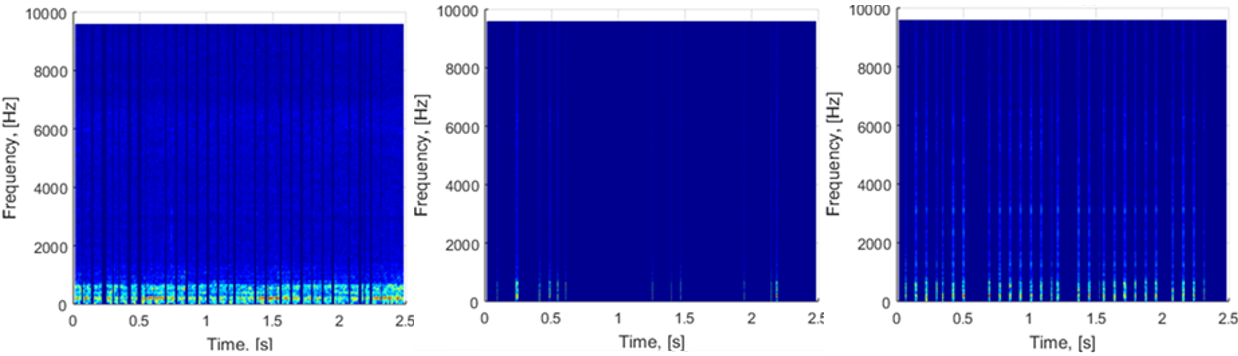
\includegraphics[width = \textwidth]{wykresy/nmf_partial.png}
\caption{Partial spectrograms constructed based on~clustering results. Third spectrogram is~selected for further analysis.}
\label{fig: nmf_partial}
\end{figure}

The methodology is~based on~nonnegative matrix factorization of~the~spectrogram, but it~should be~mentioned that the~algorithm can be~applied to~other multidimensional representations of~the~input signal. 

\begin{figure}[ht!]
\centering
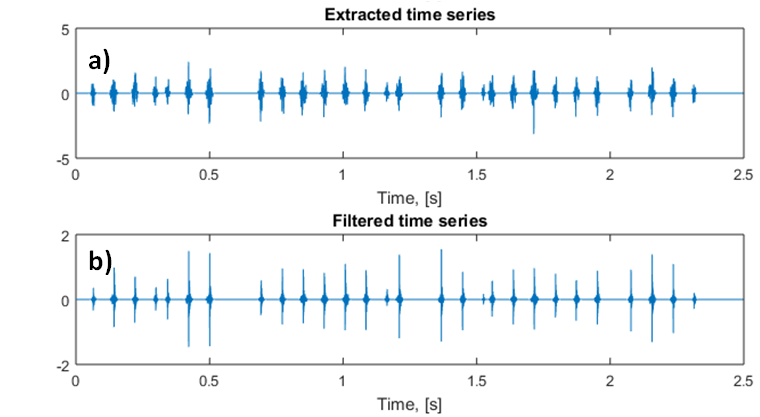
\includegraphics[width = 0.8\textwidth]{wykresy/nmf_out.png}
\caption{Recovered time series: a) after ISTFT transformation from selected partial spectrogram, b) after further highpass filtration.}
\label{fig: nmf_out}
\end{figure}

To extract proper shape of~the~impulse we perform filtration of~obtained signal with finite impulse response (FIR) highpass filter using the~Kaiser window with the~cutoff frequency equal to~1300 Hz (obtained as~optimal for maximizing SNR value), the~stopband attenuation of~-15 dB (parameters optimized for the~highest SNR). It removes low-frequency high-energy components from the~signal, and retains the~information about the~actual impulse (see Fig. \ref{fig: nmf_imp} b).

\begin{figure}[ht!]
\centering
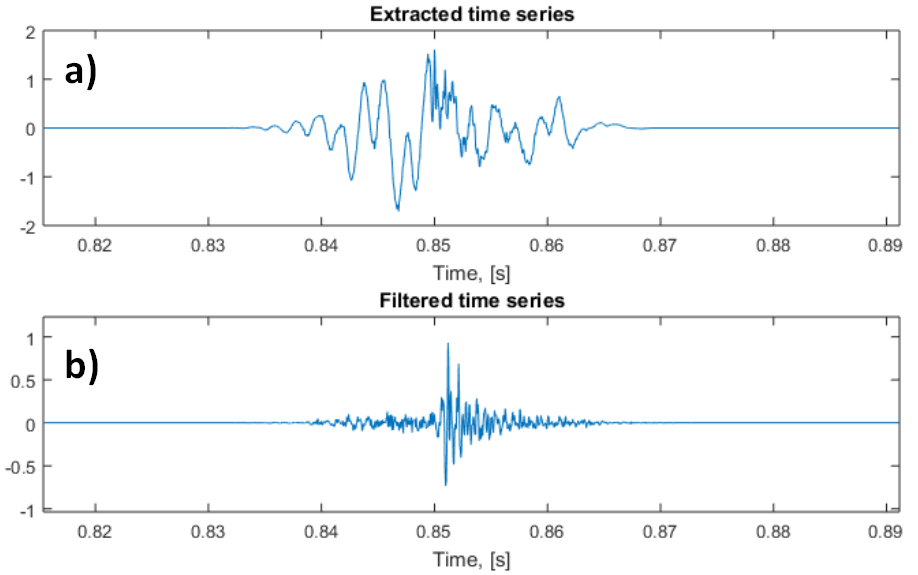
\includegraphics[width = 0.7\textwidth]{wykresy/nmf_imp.png}
\caption{Example of~impulse shape before and after filtration.}
\label{fig: nmf_imp}
\end{figure}

Obtained filtered signal contains detected impulses caused by~local damage of~the~bearing (see Fig. \ref{fig: nmf_out} b). Further analysis of~signal structure (e.g. spectral analysis) and correlating the~results with the~knowledge about the~machine kinematics can provide information leading to~identification of~precise origin of~the~damage.

\subsection{STFT analysis taking advantage of~NMF base matrix}\label{result_base}

In this section author presents the~application of~extraction method proposed in~section \ref{met_nmf_base} to~the~real-life vibration signal from copper ore crusher operating in~mining industry. 


% Since there was no available signal from faulty crusher (all machines turned out to~be in~good technical condition), an~artificial damage has been introduced to~healthy signal to~simulate cyclic damage. Component has been introduced in~a~way that it~is~not directly visible in~the~time series (Fig. \ref{fig: nmfb_raw}) or in~the~envelope spectrum (Fig. \ref{fig: nmfb_widma} top).

\begin{figure}[!ht]
\centering
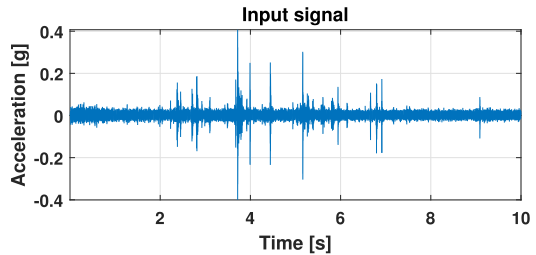
\includegraphics[width = 0.7\textwidth]{wykresy/nmfb_raw}
\caption{Input vibration signal of~the~ore crusher}
\label{fig: nmfb_raw}
\end{figure}

In Fig. \ref{fig: nmfb_raw} input vibration signal is~presented. Time series reveals numerous high-energy wideband impulses being the~result of~rocks falling into the~machine. On the~other hand, cyclic damage component is~barely noticeable above the~noise floor. Parameters of~spectrogram calculated for this dataset are presented in~Table \ref{tab:tab2}.Time-frequency representation of~data is~presented in~Fig. \ref{fig: nmfb_spec}.


\begin{table}[ht!]
  \centering
  \caption{Parameters of~spectrogram}
 \begin{tabular}{|l|l|}
  \hline
  \textbf{Parameter} & \textbf{Value} \\ \hline
     Signal length & 10 second (240000 samples) \\ \hline
     Sampling frequency & 24000 Hz \\ \hline
     Window & Hamming, 256 samples \\ \hline
     Overlap & 215 samples \\ \hline
     FFT points & 512 samples \\ \hline
     Spectrogram size & $257 \times 6404$ \\

  \hline
  \end{tabular}
  \label{tab:tab2}
\end{table}

One can notice heavy impulses across almost entire frequency dimension, while the~cyclic component is~weak and located in~the~frequency band roughly between 2200 Hz and 4800 Hz. Hence real signal is~more complicated in~its structure than the~simulated one, the~optimal amount of~clusters had to~be evaluated.

\begin{figure}[!ht]
\centering
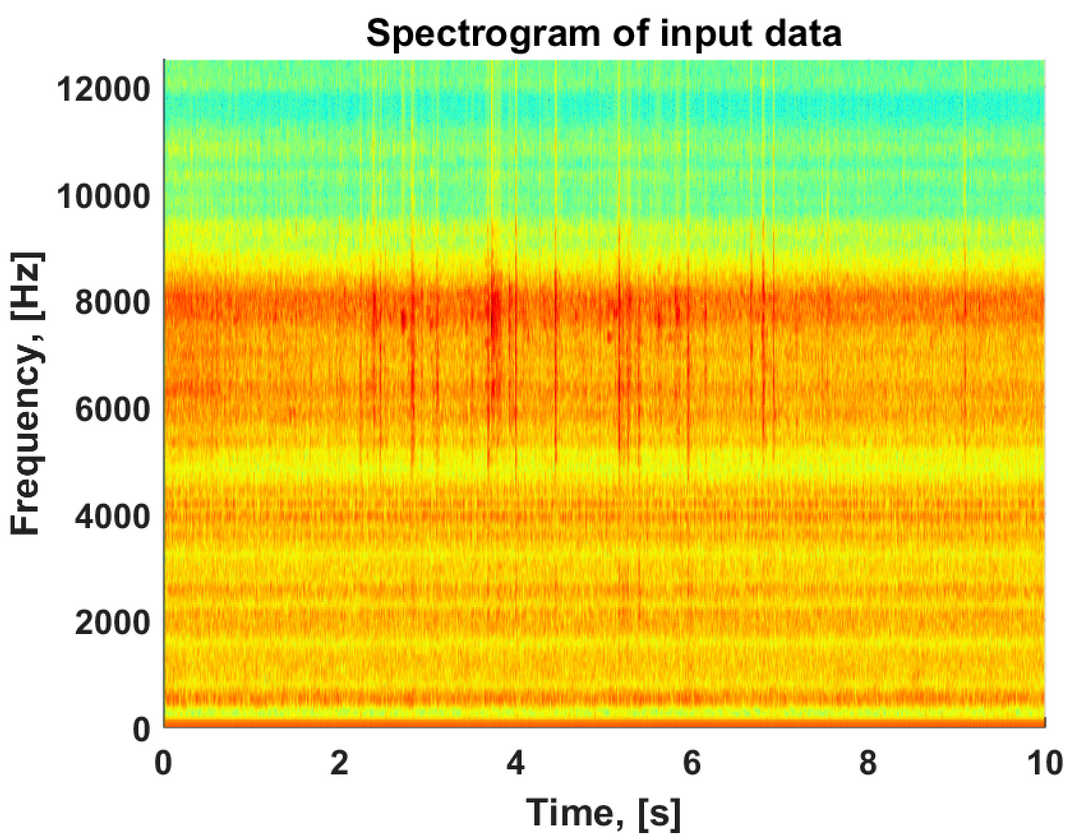
\includegraphics[width = 0.6\textwidth]{wykresy/nmfb_spec}
\caption{Time-frequency representation of~the~input signal from the~ore crusher}
\label{fig: nmfb_spec}
\end{figure}

According to~Silhouette criterion (see section \ref{app_sil}) \cite{kaufman2009finding,rousseeuw1987silhouettes}, the~optimal number of~groups is~6. The real signal is~complex and contains more different components, therefore it~is~reasonable to~use more clusters than in~simulated data.

\begin{figure}[!ht]
\centering
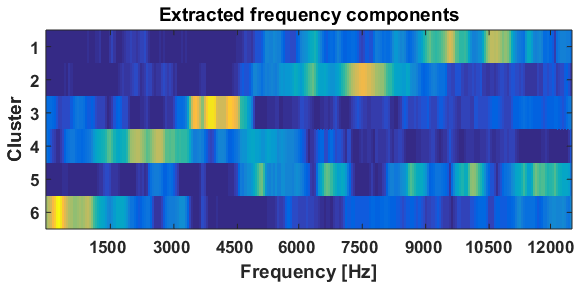
\includegraphics[width = 0.7\textwidth]{wykresy/nmfb_profiles}
\caption{Matrix W containing IFB selectors obtained by~NMF for the~ore crusher}
\label{fig: nmfb_profiles}
\end{figure}

In the~next step spectrogram matrix of~the~signal has been provided to~the~NMF algorithm for selector extraction (see Fig. \ref{fig: nmfb_profiles}). From the~point of~view of~presented research two selectors are especially interesting: the~one for non-cyclic impulses describing rock impacts, and the~one for cyclic impulsive component describing the~damage. Regarding obtained results, they are the~classes no. 2 and 3 respectively. Fig. \ref{fig: nmfb_filt} shows the~same data in~the~form of~plots.

\begin{figure}[!ht]
\centering
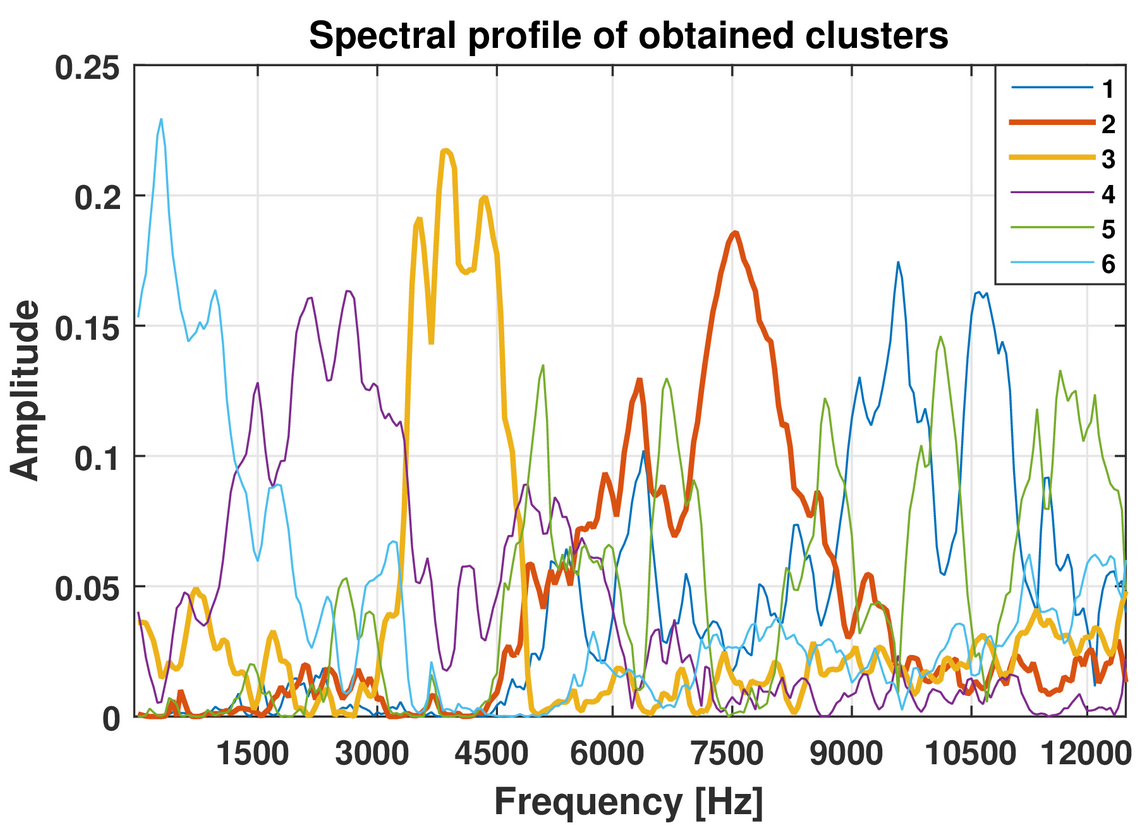
\includegraphics[width = 0.7\textwidth]{wykresy/nmfb_filt}
\caption{Plot of~IFB selectors for detected components for the~ore crusher}
\label{fig: nmfb_filt}
\end{figure}

Selection of~classes has been done using kurtosis. After its evaluation for each cluster, 2 components with greatest values (produced by~filters 2 and 3) are selected for final evaluation. Fig. \ref{fig: nmfb_out} shows the~results of~filtration.

% \begin{figure}[!ht]
% \centering
% 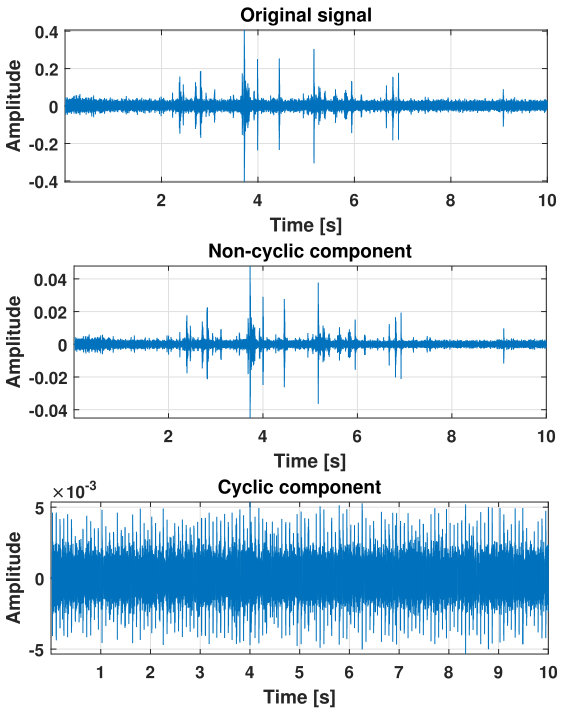
\includegraphics[width = 0.6\textwidth]{wykresy/nmfb_out}
% \caption{Results of~filtration for the~ore crusher. Top: original signal, middle: non-cyclic component, bottom: cyclic component}
% \label{fig: nmfb_out}
% \end{figure}

\begin{figure}[!ht]
 \centering
 \begin{subfigure}
   \centering
   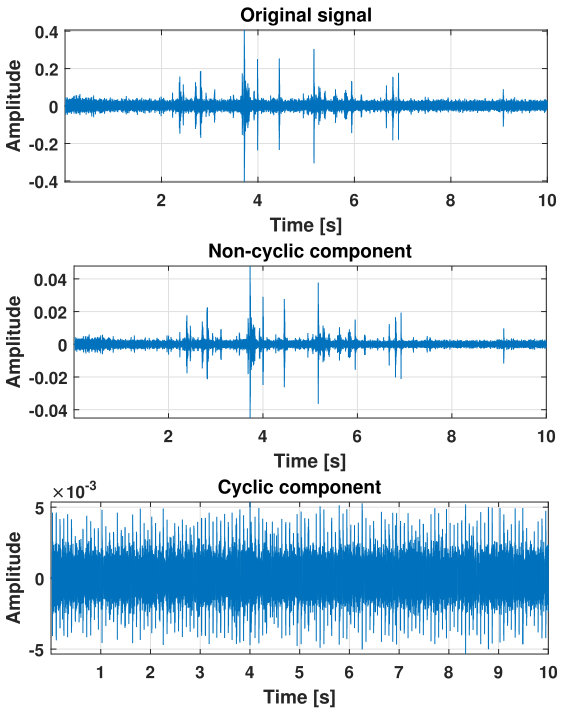
\includegraphics[width=0.48\textwidth]{wykresy/nmfb_out}
 \end{subfigure}
 \begin{subfigure}
   \centering
		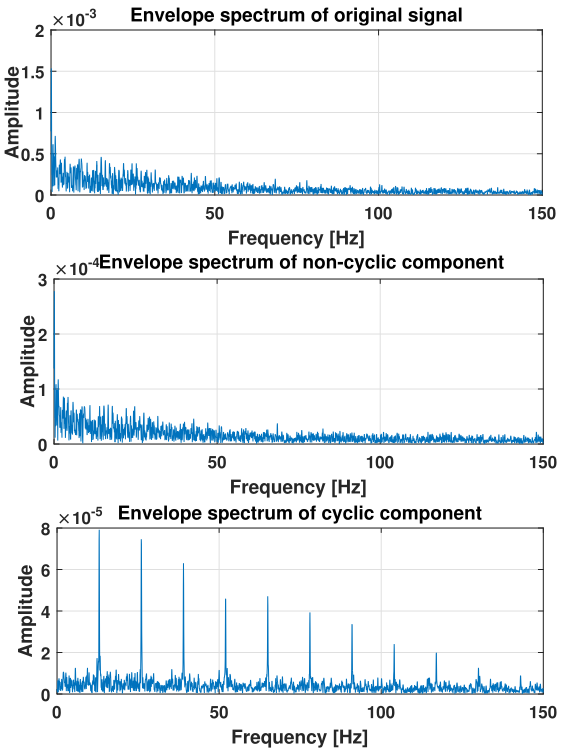
\includegraphics[width=0.45\textwidth]{wykresy/nmfb_widma}
 \end{subfigure}
 \caption{Results of~filtration for the~ore crusher. Top: original signal, middle: non-cyclic component, bottom: cyclic component}
 \label{fig: nmfb_out}
\end{figure}

As one can see, in~case of~input signal the~damage is~not visible either in~the~time series, or in~the~envelope spectrum (Fig. \ref{fig: nmfb_out} top). It is~very clear that overwhelming fraction of~the~signal information content is~occupied by~non-cyclic impulses as~well as~background components, since time series as~well as~envelope spectrum look almost exactly the~same for input signal and for extracted non-cyclic component (see Fig. \ref{fig: nmfb_out} middle).

On the~other hand, initially invisible damage component is~successfully extracted (Fig. \ref{fig: nmfb_out} bottom) and its envelope spectrum reveals clear information about the~fundamental and harmonic frequencies of~the~damage. IFB determined for this component spans the~frequencies between 3370 Hz and 4736 Hz of~the~carrier (see Fig. \ref{fig: nmfb_filt}).

% \begin{figure}[!ht]
% \centering
% 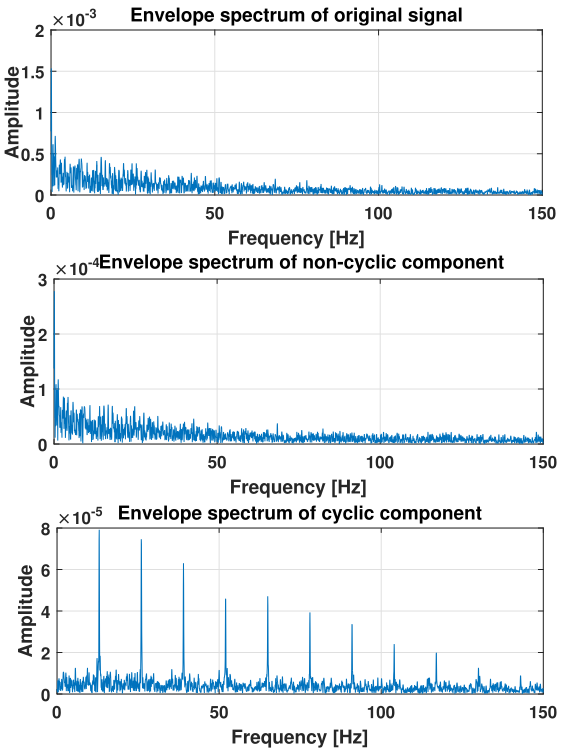
\includegraphics[width = 0.5\textwidth]{wykresy/nmfb_widma.png}
% \caption{Envelope spectra of~the~results for the~ore crusher: a) original signal, b) non-cyclic component, c) cyclic component}
% \label{fig: nmfb_widma}
% \end{figure}

\subsection{CSC analysis taking advantage of~complete NMF output}\label{result_both}

In this section author presents the~application of~extraction method proposed in~section \ref{met_nmf_both} to~the~real-life vibration signal from reciprocating gas compressor operating in~oil extraction industry.

\subsubsection{Stage 1: Preconditioning}

Figure \ref{fig:csc_raw_spec} presents the~spectrogram of~input data shown in~Figure \ref{fig:csc_raw}. While shaft-related cyclic behavior is~noticeable, SOI-related periodicity is~not detectable based on~such representation. The same result can be~observed in~the~envelope spectrum of~the~signal (see Fig. \ref{fig:csc_raw_env}), which is~the~reason of~employing different domain.

\begin{figure}[ht!]
\centering
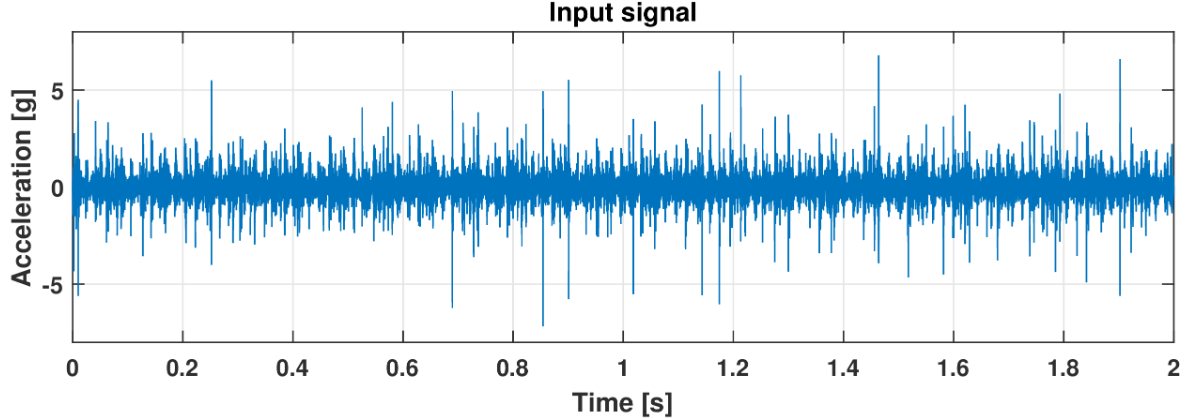
\includegraphics[width=0.8\textwidth]{wykresy/csc_raw}
\caption{Raw vibration data}
\label{fig:csc_raw}
\end{figure}

\begin{figure}[ht!]
\centering
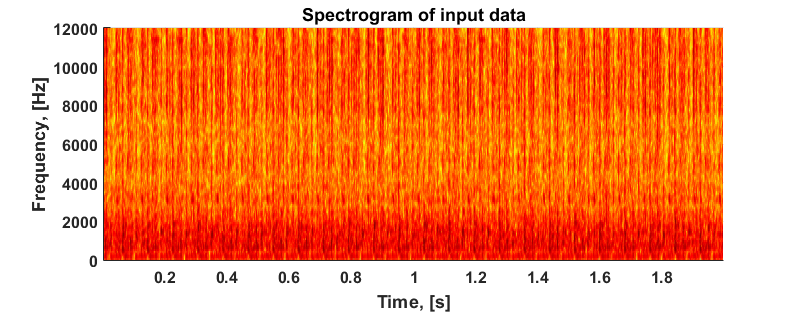
\includegraphics[width=0.8\textwidth]{wykresy/csc_raw_spec.png}
\caption{Spectrogram of~the~input vibration data}
\label{fig:csc_raw_spec}
\end{figure} 

\begin{figure}[ht!]
\centering
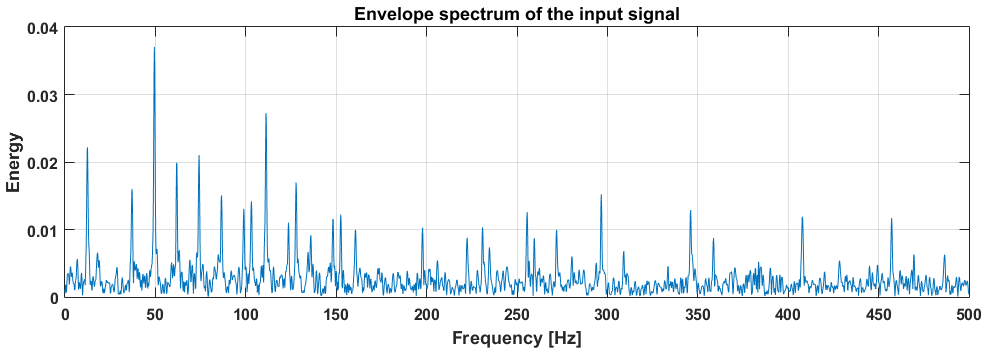
\includegraphics[width=0.8\textwidth]{wykresy/csc_raw_env.png}
\caption{Envelope spectrum of~the~input vibration data}
\label{fig:csc_raw_env}
\end{figure}

Firstly, CSC map is~calculated (see Fig. \ref{fig:csc}) from the~input signal. After primary factorization with NMF algorithm set to~2 classes, author takes advantage of~base matrix that contains set of~filters calculated for this particular CSC map. Figure \ref{fig:csc_trans} presents it~on~bottom left panel as~a~two-row matrix with carrier frequency axis common for filter bank and CSC map. On the~right panels filters are drawn conventionally. 

\begin{figure}[ht!]
\centering
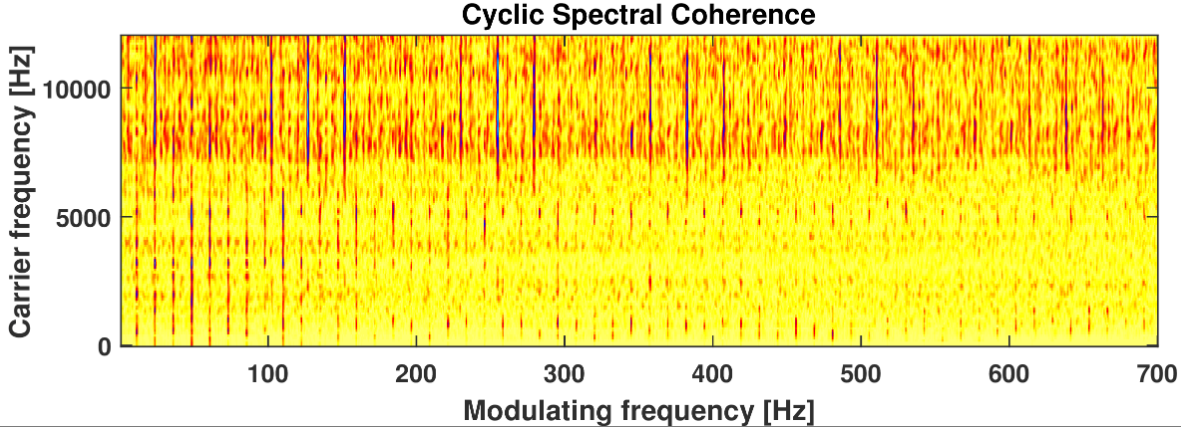
\includegraphics[width=0.8\textwidth]{wykresy/csc}
\caption{Cyclic Spectral Coherence map for the~first stage}
\label{fig:csc}
\end{figure}



\begin{figure}[ht!]
\centering
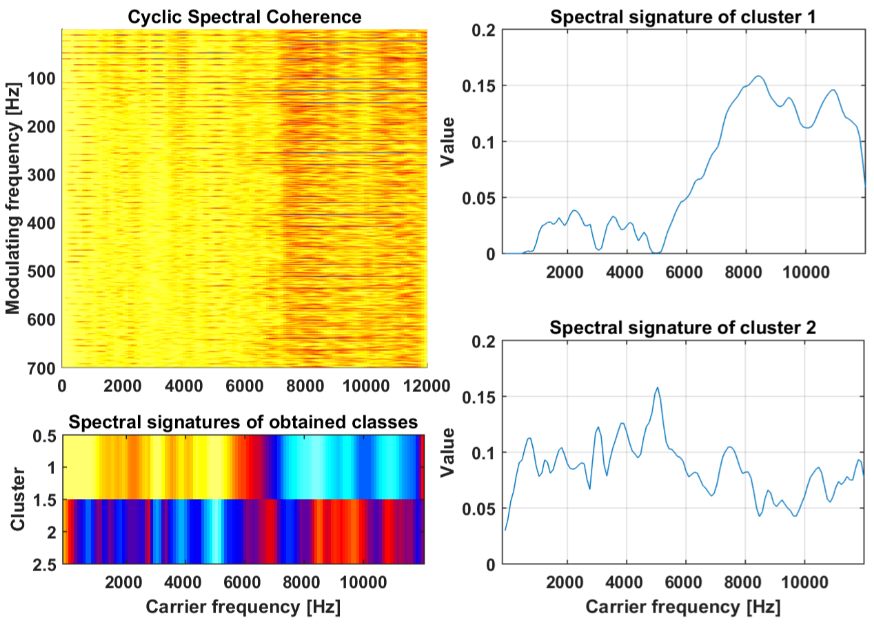
\includegraphics[width=0.8\textwidth]{wykresy/csc_trans}
\caption{Construction of~filter bank using NMF base matrix}
\label{fig:csc_trans}
\end{figure}

After that input signal is~filtered with every filter from the~bank (Figure \ref{fig:csc_out} left panels) and envelope spectra of~obtained output signals are calculated for the~evaluation of~spectral structure (Figure \ref{fig:csc_out} right panels). Envelope spectrum of~the~second cluster contains fundamental frequency component of~$12,35$ Hz and its harmonics that are the~indicators of~the~rotational speed of~the~compressor shaft. On the~other hand, the~first cluster reveals the~fundamental frequency of~$127,9$ Hz and its harmonics, that additionally occur with very regular sidebands. Fundamental frequency perfectly corresponds with the~expected frequency of~BPFI for this bearing, while the~presence of~sidebands suggests the~cyclic modulation in~the~signal that is~also very common in~cases of~local damage in~rotating elements. It is~easy to~conclude that this is~the~cluster of~interest, but this information can be~also obtained in~an~automatic way by~finding a~cluster with greatest SNR of~the~time series. Note that the~change of~scale in~the~time series for obtained clusters (scaling of~vertical axis) occurs due to~characteristic of~the~filter, that even in~the~passband takes the~values less then one, however it~does not affect the~structure of~the~signal but only its amplitude.

\begin{figure}[ht!]
\centering
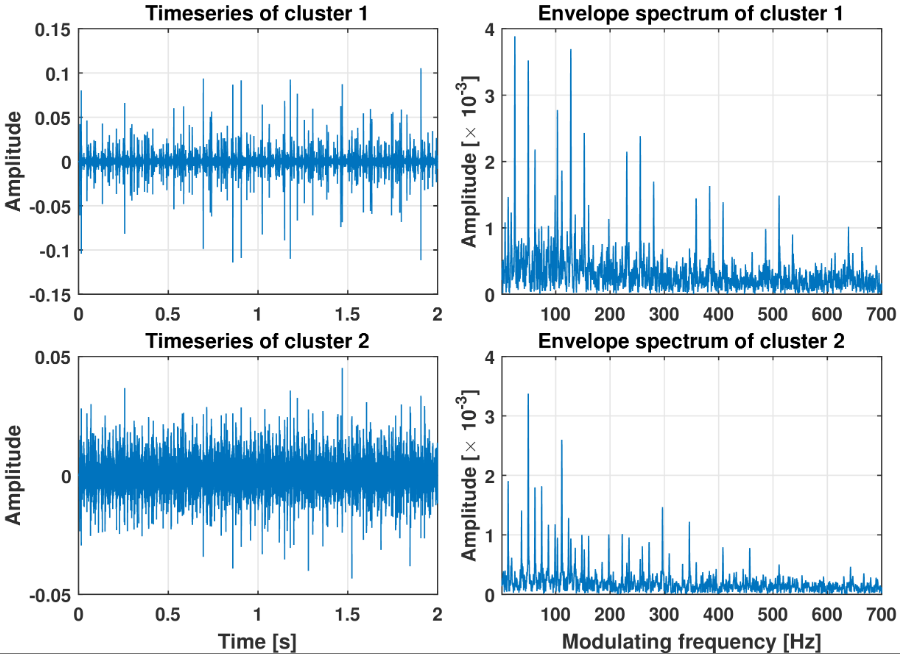
\includegraphics[width=0.7\textwidth]{wykresy/csc_out}
\caption{Results of~method operation. Left panels: extracted time series, right panels: corresponding envelope spectra.}
\label{fig:csc_out}
\end{figure}

\subsubsection{Stage 2: Enhancement}

While for experienced user it~could be~possible to~identify the~character of~the~damage already, envelope spectrum is~still not very clean and a~lot of~different frequency components are present, especially within lower frequency bands and in~terms of~significant background noise. Hence, the~second stage of~presented methodology is~expected to~clean the~signal by~spatial denoising of~CSC map.

\begin{figure}[ht!]
\centering
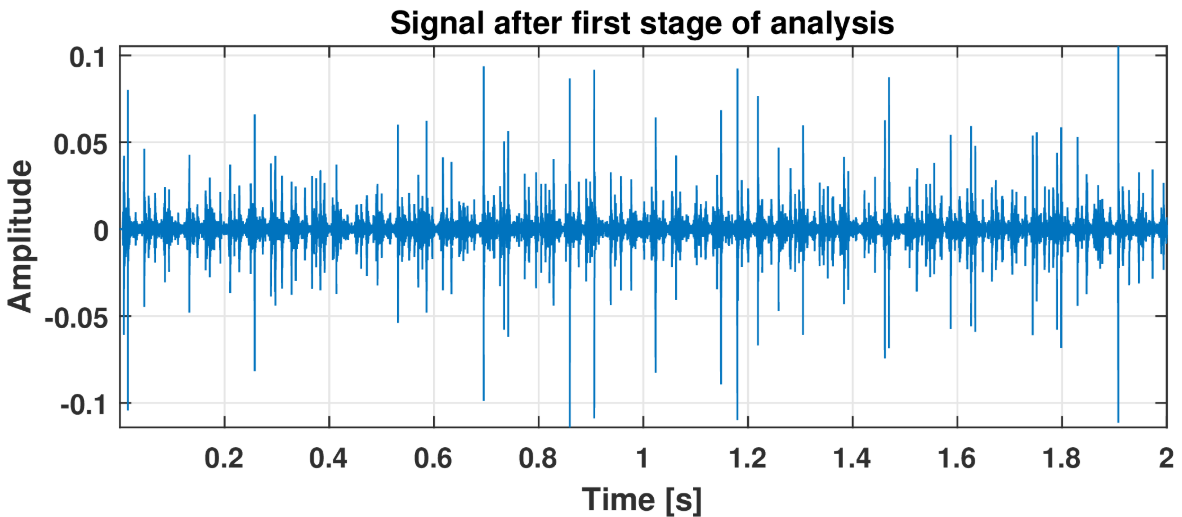
\includegraphics[width=0.6\textwidth]{wykresy/csc_raw2}
\caption{Input signal for the~second stage}
\label{fig:csc_raw2}
\end{figure}

Input signal for this stage (being the~time series of~first cluster from first stage of~analysis, see Figure~\ref{fig:csc_raw2}) is~decomposed into CSC map of~its own (see Figure~\ref{fig:csc_csc2}). After that spatial noise model matrix is~constructed according to~description in~section~\ref{denoise} (see Figure~\ref{fig:csc_spd}) and subtracted from CSC map. This way it~is~possible to~present and utilize new denoised CSC map, that is~provided for the~third stage of~analysis (see Figure~\ref{fig:csc_csc3}).

\begin{figure}[ht!]
\centering
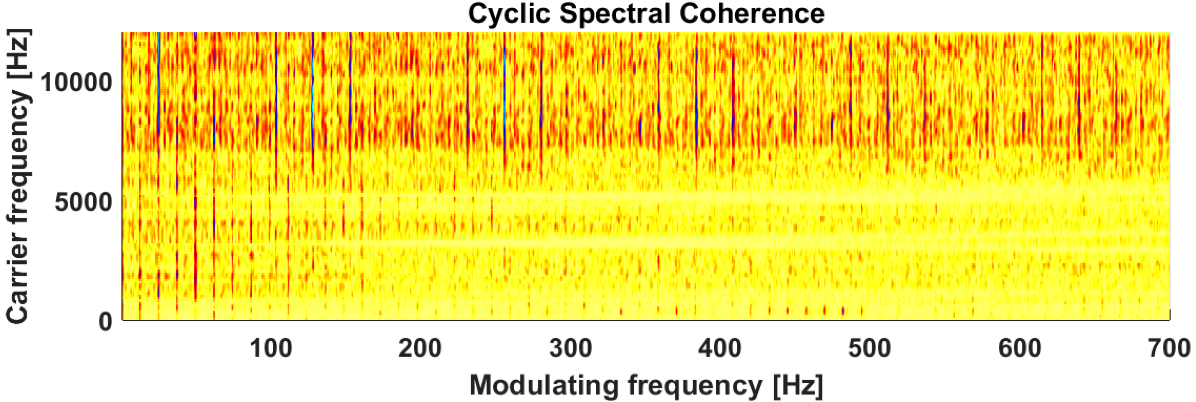
\includegraphics[width=0.8\textwidth]{wykresy/csc_csc2}
\caption{Cyclic Spectral Coherence map for the~second stage}
\label{fig:csc_csc2}
\end{figure}

\begin{figure}[ht!]
\centering
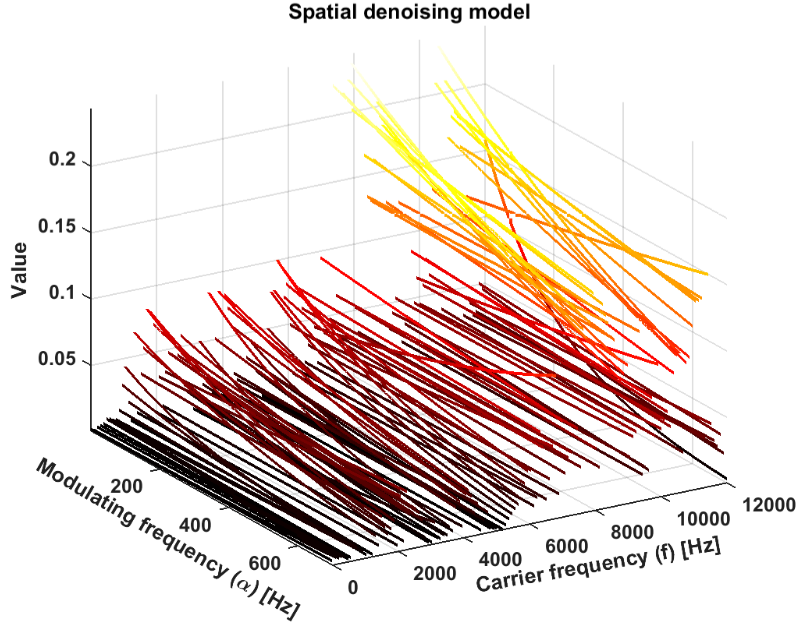
\includegraphics[width=0.7\textwidth]{wykresy/csc_spd}
\caption{Spatial denoising model}
\label{fig:csc_spd}
\end{figure}

\begin{figure}[ht!]
\centering
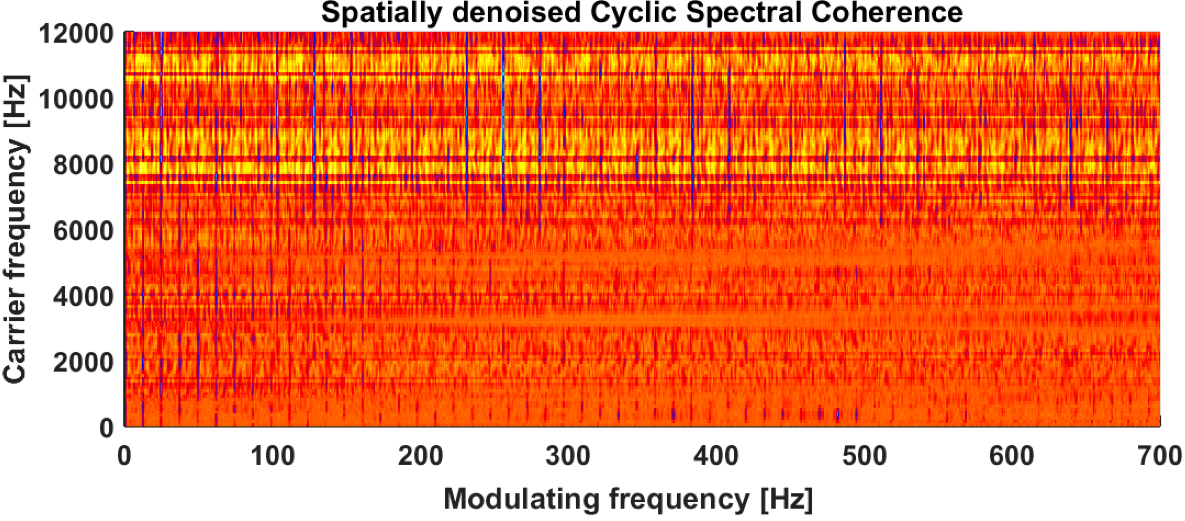
\includegraphics[width=0.7\textwidth]{wykresy/csc_csc3}
\caption{Spatially denoised Cyclic Spectral Coherence map}
\label{fig:csc_csc3}
\end{figure}

\subsubsection{Stage 3: Extraction}

At this point third stage of~analysis begins, majority of~which is~focused on~Monte Carlo iterations described in~detail in~section \ref{mcmc}. For the~purpose of~robustness NMF factorization in~this stage was set to~six classes. Figure \ref{fig:csc_enc} presents the~example of~how classes might look like in~a~single MC iteration as~an~encoding matrix, and Figure \ref{fig:csc_classes} presents them as~individual plots. It is~directly the~encoding matrix of~NMF, but its vectors are presented on~individual plots. It is~visible that top-center ($2^{nd}$) cluster contains spectrum related to~shaft rotation and bottom-left ($4^{th}$) cluster stands for the~damaged bearing signature. However, it~is~clear that in~this example spectra are not selected perfectly, which is~very common effect, easiest observable on~the~damage cluster. Desired cluster describing damage spectrum is~automatically selected with maximum value of~kurtosis of~spectrum vector. 

\begin{figure}[ht!]
\centering
\includegraphics[width=0.8\textwidth]{wykresy/csc_enc2}
\caption{Example of~encoding matrix produced by~NMF in~a~single Monte Carlo iteration}
\label{fig:csc_enc}
\end{figure}

\begin{figure}[ht!]
\centering
\includegraphics[width=0.8\textwidth]{wykresy/csc_clusters}
\caption{Example classes produced by~NMF in~a~single Monte Carlo iteration, numbers in~panel titles indicate cluster kurtosis}
\label{fig:csc_classes}
\end{figure}

Figure \ref{fig:csc_multi} presents examples of~damage cluster properly selected in~consecutive MC iterations. As explained before, those clusters will not be~identical, but most of~the~time they are mostly correct, which is~why MC technique is~used to~mitigate this effect. Finally median of~selected clusters is~calculated to~extract common components. Envelope spectrum obtained that way is~a~perfect representation of~frequency components related to~damage (see Figure \ref{fig:csc_out2}).

\begin{figure}[ht!]
\centering
\includegraphics[width=0.7\textwidth]{wykresy/csc_multi}
\caption{Examples of~selected clusters}
\label{fig:csc_multi}
\end{figure}

Note that the~amplitudes of~components are much higher in~comparison to~the~envelope spectra presented in~earlier stages of~the~method. This effect occurs because of~the~fact that presented final envelope spectrum is~in~fact obtained by~the~sum of~correlation coefficients across the~CSC map. Hence, those summation can produce such high values. As it~was stated before, the~goal is~to~obtain clear pattern (fault frequencies surrounded by~the~sidebands with no additional noise floor).

\begin{figure}[ht!]
\centering
\includegraphics[width=0.7\textwidth]{wykresy/csc_out2}
\caption{Final damage component envelope spectrum}
\label{fig:csc_out2}
\end{figure}

\clearpage
\section{Automatic information extraction with Progressive Genetic Algorithm}\label{results_pga}

In this chapter the~application of~the~methodology described in~section \ref{met_pga} to~real and simulated data is~presented. Author evaluates performance of~the~algorithm using real-life data from damaged bearing. Parameters of~designed real-coded progressive genetic algorithm (PGA) are presented in~Table \ref{tab:tab3}.

\begin{table}[ht!]
  \centering
  \caption{Parameters of~PGA}
  \begin{tabular}{|l|l|}
  \hline
     \textbf{Parameter} & \textbf{Value} \\ \hline
     Initial filter length & 7 \\ \hline
     Population size & 150 \\ \hline
     Termination criterion & NRMSE \\ \hline
     Generations per epoch & 80 \\ \hline
     Initial population & Random $\sim$ N(0,1) \\ \hline
     Selection & Roulette \\ \hline
     Crossover & Heuristic with d=1.5 \\ \hline
     Mutation & Uniform with R=0.01 \\ \hline
     Stall limit & 20 \\ \hline
     Average change for stall limit & $10^{-6}$ \\ \hline
     Elite individuals & 3 \\
  \hline
  \end{tabular}
  \label{tab:tab3}
\end{table}

Author analyzes one-dimensional vibration signal acquired on~rolling ball bearing of~the~drive pulley operating in~belt conveyor driving station. Sampling frequency is~equal to~19.2 kHz. Fig. \ref{fig:gb} presents the~described gearbox and in~Fig. \ref{fig:pga_raw} time series of~signal is~presented. Signal is~known to~contain wideband impulses with modulation frequency 12.7 Hz corresponding to~outer race local damage. More information can be~found in~other papers concerning the~diagnostics of~this machine \cite{zimroz2009some}. Kurtosis value for this sample is~equal to~3.09.

\begin{figure}[ht!]
\centering
\includegraphics[width=0.7\textwidth]{wykresy/pga_raw.png}
\caption{Raw input signal}
\label{fig:pga_raw}
\end{figure}

\subsubsection{Results}

General results of~the~algorithm operation are presented in~Fig. \ref{fig:pga_real1}. One can see that input signal (Fig. \ref{fig:pga_real1}a) processed with obtained filter reveals damage-related impulses in~a~very clear way, achieving kurtosis value of~87.23, which denotes the~improvement by~2722$\%$ (Fig. \ref{fig:pga_real1}d). Such high ratio (nearly 30 times higher than the~original value) can be~the~first indication of~the~presence of~local damage. Envelope spectrum of~input and output signal are presented in~Fig. \ref{fig:pga_real1}b and \ref{fig:pga_real1}e respectively. Spectrograms of~input and output signals (Fig. \ref{fig:pga_real1}c and \ref{fig:pga_real1}f respectively) present the~time-frequency structure comparison between them and evaluate the~obtained IFB. Frequency response shows that optimization process created the~filter that turned out to~be arbitrarily custom and practically impossible to~obtain by~manual design (Fig. \ref{fig:pga_real2}c). Phase linearity within passbands also has been achieved, which is~essential for distortion avoidance (Fig. \ref{fig:pga_real2}d). Vector of~obtained filter coefficients is~presented in~Fig. \ref{fig:pga_real2}a). 

\begin{figure}[ht!]
\centering
\includegraphics[width=0.8\textwidth]{wykresy/pga_real1.png}
\caption{Comparison between real-life input and output signals describing damaged bearing: a) time series of~input signal, d) time series of~filtered signal, b) envelope spectrum of~input signal (60 Hz component and its multiples are the~harmonic frequencies of~a~power grid), e) envelope spectrum of~output signal (12.7 Hz component and its multiples are related to~damage of~the~bearing), c) spectrogram of~input signal, f) spectrogram of~output signal}
\label{fig:pga_real1}
\end{figure}

Even brief visual inspection if the~coefficients can provide information about some underlying low-cut character of~the~filter, which is~very important for suppressing low-frequency high-energy components present in~the~input signal.

Fig. \ref{fig:pga_real2}b) presents the~progression of~kurtosis value being the~fitness function for the~GA. Two main aspects of~this curve can be~distinguished:

\begin{itemize}
  \item jagged growth,
  \item points of~decreasing value occurring occasionally throughout the~whole process.
\end{itemize}

\begin{figure}[ht!]
\centering
\includegraphics[width=0.8\textwidth]{wykresy/pga_real2.png}
\caption{Final results of~filter optimization for real-life damaged case: a) vector of~filter coefficients, b) fitness progression, c) magnitude response of~obtained filter, d) phase response of~obtained filter}
\label{fig:pga_real2}
\end{figure}


\begin{figure}[ht!]
\centering
\includegraphics[width=0.5\textwidth]{wykresy/pga_real3.png}
\caption{Values of~termination function for real signal.}
\label{fig:pga_real3}
\end{figure}

Jagged growth is~the~first inherent property of~the~progressiveness of~GA. At the~beginning filter is~short and its fitness value is~not expected to~be very high. It improves within a~single epoch, but not by~far. In the~next epoch filter becomes longer, which rapidly increases its capability to~achieve better fitness. Extending filter length provides more progress than optimization within a~single epoch, but for the~reasons explained in~section \ref{pga} this is~essential for overall outcome and algorithm should not begin the~operation with longer filter in~the~first place. Points of~decreasing fitness value are another inherent property of~GA progressiveness. This effect, every time it~occurs, lasts only one generation being the~consequence of~filter prolonging operation. When new epoch begins, two additional coefficients are appended to~the~coefficient vector. Since those values are random, most of~the~time filter turns out to~be worse than the~last one from the~previous epoch, and its fitness is~lower. After that, in~the~next generation algorithm recognizes new possibilities and requires one or two generations to~evolve the~filter higher than ever before, continuing the~overall optimization process. Termination function values are presented in~Fig. \ref{fig:pga_real3}. Final value that algorithm terminates at, is~equal to~2.06, which is~the~first value of~NRMSE that dropped below the~5$\%$ threshold.

\subsubsection{Discussion}

In machine diagnostics, obtaining decision about the~technical condition of~investigated machine is~the~final objective. In presented methodology one can observe strong correlation between kurtosis value after filtration and actual information about present damage. Hence, it~is~proposed to~establish threshold of~fitness value equal to~100$\%$ increase (200$\%$ of~initial value). Results with fitness value lower than proposed level would be~labeled as~healthy, and higher – as~damaged. In presented research damaged cases reached levels of~nearly 3000$\%$ and nearly 400$\%$, and healthy case reached only 1$\%$ of~increase.

\subsubsection{Comparison with classical methods}

One of~the~most recognized methods for IFB determination is~filtration using filter determined by~kurtogram \cite{antoni2007fast}. The kurtogram is~a~fourth-order spectral analysis tool elaborated for detecting and characterising nonstationarities in~a~signal. It relies on~the~assertion that each type of~transient is~associated with an~optimal frequency/frequency resolution dyad (\textit{f}; $\delta$\textit{f}) which maximises the~kurtosis.

Another method used for comparison is~spectral kurtosis introduced by~Antoni and Randall \cite{antoni2006spectral} is~regarded as~one of~the~most powerful and popular approaches to~localize informative frequency band, especially for vibration signal analysis \cite{randall2011rolling}. The general principle of~operation is~to~calculate kurtosis value for each frequency bin of~the~spectrogram (\ref{eq:kurtosis}). As a~result, one can obtain indicator of~impulsiveness across the~signal spectrum, which allows to~determine which frequency bands carry the~most visible information about the~damage-related impulsive behavior. Vector of~spectral kurtosis can be~then used as~a~filter to~extract those impulsive components from the~signal.



% \begin{figure}[ht!]
% \centering
% \includegraphics[width=0.9\textwidth]{wykresy/SK.png}
% \caption{Spectral Kurtosis function for real signal.}
% \label{fig:SK}
% \end{figure}



\begin{figure}[!ht]
 \centering
 \begin{subfigure}
   \centering
   \includegraphics[width=0.45\textwidth]{wykresy/SK}
 \end{subfigure}
 \begin{subfigure}
   \centering
		\includegraphics[width=0.45\textwidth]{wykresy/kurtogram}
 \end{subfigure}
 \caption{Selectors used for comparison: Spectral Kurtosis (left panel) and kurtogram (right panel)}
 \label{fig:comps}
\end{figure}


As a~point of~reference, author compares the~results to~filtration based on~SK and kurtogram for real industrial signal. It is~important to~mention at~this point that for method comparison authors use envelopes because the~way that kurtogram is~calculated only allows to~obtain envelope after filtration. Spectral kurtosis function for this data is~presented in~the~left panel of~Fig. \ref{fig:comps}, and kurtogram in~the~right panel of~Fig. \ref{fig:comps}. Envelopes of~raw signal filtered with all three methods are presented in~Fig. \ref{fig:comp}. In this comparison envelopes are used, since for the~way that kurtogram filtering is~implemented, only signal envelope is~possible to~be obtained. It can be~easily seen that signal filtered with SK is~characterized with much stronger noisefloor than after filtration with evolved filter or kurtogram-based filter. That causes weaker impulses to~be lost in~noise. Furthermore, kurtosis and Signal-to-Noise Ratio (SNR) values are also a~lot lower than for presented method and kurtogram method.

% Initial signal (Envelope kurtosis=3,56) filtered with SK is~characterized with envelope kurtosis value equal to~38, filtered with Kurtogram-based filter while after filtering with evolved filter kurtosis rises up to~87,23 (and even higher, if longer filter evolution were allowed).

\begin{table}[ht!]
  \centering
  \caption{Parameters of~compared results}
 \begin{tabular}{|l|l|l|}
  \hline
  \textbf{Method} & \textbf{Envelope kurtosis} & \textbf{Envelope SNR [dBc]} \\ \hline
     Raw signal & 3,56 & -7,1 \\ \hline
     PGA-filtered & 129 & -14,02 \\ \hline
     Kurtogram-filtered & 51 & -13,93 \\ \hline
     SK-filtered & 38 & -9,9 \\
     
  \hline
  \end{tabular}
  \label{tab:tab4}
\end{table}

% Another aspect worth noting is~the~rotational speed of~the~bearing. Presented method is~based on~the~assumption that rotational speed is~constant. Of course, authors realize that it~is~not, but the~conditions of~measurement of~real signal allow to~believe that machine was operating with quasi-constant speed for the~given period of~time. In addition, minor variations in~rotational speed are not crucial for the~performance of~this method, but for large speed fluctuation, number of~impulses might affect kurtosis and indeed it~might lead to~false results.

\begin{figure}[ht!]
\centering
\includegraphics[width=0.8\textwidth]{wykresy/comp.png}
\caption{Comparison of~envelopes of~signals after filtration with PGA filter (top panel), using kurtogram (middle panel) and using spectral kurtosis (bottom panel)}
\label{fig:comp}
\end{figure}




